% !TeX program = xelatex
\documentclass[a4paper,12pt]{article}

% ============================================================================
% កញ្ចប់បណ្ណាល័យ និងរចនាប័ទ្ម Mobile-First Readability (NGS Preah Krasang)
% ============================================================================
\usepackage[a4paper, left=1.45cm, right=1.45cm, top=2.30cm, bottom=2.30cm, headheight=18pt, headsep=0.68cm, footskip=0.88cm]{geometry}
\usepackage{amsmath, amssymb}
\usepackage{unicode-math}
\usepackage{fontspec}
\usepackage{array, longtable, multirow, colortbl, booktabs}
\usepackage[table]{xcolor}
\usepackage{enumitem}
\usepackage{pifont}
\usepackage{fancyhdr}
\usepackage{lastpage}
\usepackage{needspace}
\usepackage[hyphens]{url}
\usepackage{tikz}
\usetikzlibrary{calc, arrows.meta, decorations.markings, decorations.pathreplacing, positioning, babel}
\usepackage[most]{tcolorbox}
\tcbuselibrary{breakable, skins}
\urlstyle{same}

% LaTeX 2025 + longtable v4.24 compatibility guard
\makeatletter
\let\@expl@@@mark@update@singlecol@structures@@\relax
\makeatother

% ============================================================================
% ការកំណត់ពុម្ពអក្សរ (Cross-Platform Fonts Configuration)
% ============================================================================
\providecommand{\NGSFindFonts}{%
  \IfFileExists{C:/Windows/Fonts/cambria.ttc}{%
    \def\NGSSysPath{C:/Windows/Fonts/}%
    \def\NGSUserPath{C:/Users/KIT/AppData/Local/Microsoft/Windows/Fonts/}%
  }{%
    \IfFileExists{./fonts/KhmerOSsiemreap.ttf}{\def\NGSSysPath{./fonts/}\def\NGSUserPath{./fonts/}}{%
    \IfFileExists{../fonts/KhmerOSsiemreap.ttf}{\def\NGSSysPath{../fonts/}\def\NGSUserPath{../fonts/}}{%
    \IfFileExists{../../fonts/KhmerOSsiemreap.ttf}{\def\NGSSysPath{../../fonts/}\def\NGSUserPath{../../fonts/}}{%
    \IfFileExists{../../../fonts/KhmerOSsiemreap.ttf}{\def\NGSSysPath{../../../fonts/}\def\NGSUserPath{../../../fonts/}}{%
    \IfFileExists{../../../../fonts/KhmerOSsiemreap.ttf}{\def\NGSSysPath{../../../../fonts/}\def\NGSUserPath{../../../../fonts/}}{%
    \IfFileExists{../../../../../fonts/KhmerOSsiemreap.ttf}{\def\NGSSysPath{../../../../../fonts/}\def\NGSUserPath{../../../../../fonts/}}{%
    \IfFileExists{../../../../../../fonts/KhmerOSsiemreap.ttf}{\def\NGSSysPath{../../../../../../fonts/}\def\NGSUserPath{../../../../../../fonts/}}{%
      \def\NGSSysPath{../../../../../../../fonts/}\def\NGSUserPath{../../../../../../../fonts/}%
    }}}}}}}%
  }%
}
\NGSFindFonts

\setmathfont[
  Path={\NGSSysPath},
  FontIndex=1,
  Scale=1.06
]{cambria.ttc}

\defaultfontfeatures{Ligatures=TeX}

\setmainfont[
  Path={\NGSUserPath},
  Extension=.ttf,
  Script=Khmer,
  BoldFont={KhmerOSsiemreap},
  BoldFeatures={FakeBold=1.8},
  ItalicFont={KhmerOSsiemreap},
  ItalicFeatures={FakeSlant=0.25},
  BoldItalicFont={KhmerOSsiemreap},
  BoldItalicFeatures={FakeBold=1.8, FakeSlant=0.25}
]{KhmerOSsiemreap}

\newfontfamily\muol[
  Path={\NGSUserPath},
  Extension=.ttf,
  Script=Khmer
]{KhmerOSmuollight}

\newfontfamily\TimesEn[
  Path={\NGSSysPath},
  Extension=.ttf,
  Scale=1.02,
  BoldFont={timesbd},
  ItalicFont={timesi},
  BoldItalicFont={timesbi}
]{times}

\newfontfamily\NagaBold[
  Path={\NGSUserPath},
  Extension=.ttf
]{AKbalthom Naga Bold}

\newfontfamily\CalibriFont[
  Path={\NGSSysPath},
  Extension=.ttf
]{calibri}

\newfontfamily\Tacteing[
  Path={\NGSUserPath}
]{TACTENG.TTF}

\newfontfamily\CourierBullet[
  Path={\NGSSysPath},
  Extension=.ttf
]{cour}

% ក្បួនកាត់ពាក្យខ្មែរ (Khmer word wrapping)
\XeTeXlinebreaklocale "km"
\XeTeXlinebreakskip = 0pt plus 1pt minus 0.1pt

% ============================================================================
% ពណ៌ស-ខ្មៅស្តង់ដារបោះពុម្ព និងអានលើទូរស័ព្ទ (B&W Print-Safe Monochrome Palette)
% ============================================================================
\definecolor{bordergray}{HTML}{333333}
\definecolor{midgray}{HTML}{595959}
\definecolor{stepgray}{HTML}{D9D9D9}
\definecolor{bannergray}{HTML}{EAEAEA}
\definecolor{headgray}{HTML}{F0F0F0}
\definecolor{panelgray}{HTML}{F7F7F7}
\definecolor{badgegray}{HTML}{FFFFFF}

% ============================================================================
% ម៉ាក្រូអក្សរ និងទម្រង់ក្បាល/ជើងទំព័រ (Macros & Header/Footer with Struts)
% ============================================================================
\newcommand{\en}[1]{{\TimesEn #1}}
\newcommand{\enbf}[1]{{\TimesEn\bfseries #1}}
\newcommand{\enit}[1]{{\TimesEn\itshape #1}}
\newcommand{\enbi}[1]{{\TimesEn\bfseries\itshape #1}}
\newcommand{\unit}[1]{\,\text{\en{#1}}}
\newcommand{\khmflourish}{{\Tacteing\fontsize{38pt}{15pt}\selectfont\raisebox{-5pt}{3}}}
\newcommand{\ditem}{\tikz[baseline=-0.5ex]\fill (0,0.44ex) -- (0.44ex,0) -- (0,-0.44ex) -- (-0.44ex,0) -- cycle;\hspace{0.35em}}
\newcommand{\wcirc}{{\CourierBullet\fontsize{10pt}{12pt}\selectfont o}\hspace{0.25em}}
\newcommand{\cnum}[1]{{\fontsize{11pt}{13pt}\selectfont\ding{\numexpr181+#1\relax}}\hspace{0.15em}}
\newcommand{\ckmark}{\ding{51}}
\newcommand{\xkmark}{\ding{55}}
\newcommand{\tblhead}[1]{{\linespread{1.0}\muol\fontsize{10.2pt}{16pt}\selectfont #1\par}}
\newcommand{\saylead}{{\linespread{1.0}\muol\fontsize{10.8pt}{17pt}\selectfont គ្រូនិយាយថា៖}\hspace{0.35em}}
\newcommand{\figcap}[2]{%
  \par\nopagebreak\vspace{2pt}%
  {\centering\linespread{1.12}\fontsize{10.5pt}{15pt}\selectfont
    {\muol\fontsize{10.5pt}{16.5pt}\selectfont រូបទី #1៖}\hspace{0.3em}#2\par}%
  \vspace{4pt}%
}

\pagestyle{fancy}
\fancyhf{}
\renewcommand{\headrulewidth}{0.4pt}
\renewcommand{\footrulewidth}{0.4pt}
\fancyhead[L]{\rule[-3pt]{0pt}{14pt}\fontsize{9.5pt}{13.5pt}\selectfont មគ្គុទ្ទេសក៍គរុកោសល្យគ្រូ \en{(Grade 8 POW23)}}
\fancyhead[R]{\rule[-3pt]{0pt}{14pt}\fontsize{9.5pt}{13.5pt}\selectfont មេរៀនទី២ \en{(}២.៣\en{)}៖ វិធីចែកស្វ័យគុណមាននិទស្សន្តរ៉ឺឡាទីប}
\fancyfoot[L]{\rule{0pt}{13pt}\fontsize{9.5pt}{13.5pt}\selectfont កញ្ចប់ឯកសារ \en{NGS 5Es (50 min) |} ហុក ប៊ុនថែន}
\fancyfoot[R]{\rule{0pt}{13pt}\fontsize{9.5pt}{13.5pt}\selectfont ទំព័រ \en{\thepage\ / \pageref{LastPage}}}

\fancypagestyle{firstpage}{%
  \fancyhf{}%
  \renewcommand{\headrulewidth}{0pt}%
  \renewcommand{\footrulewidth}{0.4pt}%
  \fancyfoot[L]{\rule{0pt}{13pt}\fontsize{9.5pt}{13.5pt}\selectfont អនុវិទ្យាល័យព្រះក្រសាំង \en{(Preah Krasang NGS)}}%
  \fancyfoot[R]{\rule{0pt}{13pt}\fontsize{9.5pt}{13.5pt}\selectfont ទំព័រ \en{\thepage\ / \pageref{LastPage}}}%
}

% ============================================================================
% ឋានានុក្រមចំណងជើង និងប្រអប់ Mobile-First (Tier 2-3 & Breakable Boxes)
% ============================================================================
\newcommand{\secbanner}[2]{%
  \Needspace{2.2cm}%
  \begin{tcolorbox}[
    enhanced,
    colback=bannergray,
    colframe=bordergray,
    boxrule=0.9pt,
    leftrule=3.8pt,
    arc=2pt,
    top=6pt, bottom=6pt, left=9pt, right=9pt,
    before skip=10pt, after skip=6pt
  ]
    {\linespread{1.0}\muol\fontsize{12pt}{19pt}\selectfont #1}\\[-1pt]
    {\linespread{1.0}\fontsize{10pt}{14.5pt}\selectfont\enit{#2}}
  \end{tcolorbox}%
}

\newcommand{\refbanner}[1]{%
  \Needspace{2.2cm}%
  \begin{tcolorbox}[
    enhanced,
    colback=bannergray,
    colframe=bordergray,
    boxrule=0.9pt,
    leftrule=3.8pt,
    arc=2pt,
    top=6pt, bottom=6pt, left=9pt, right=9pt,
    before skip=10pt, after skip=6pt
  ]
    {\linespread{1.0}\muol\fontsize{12pt}{19pt}\selectfont #1}
  \end{tcolorbox}%
}

\newcommand{\subsec}[1]{%
  \Needspace{1.7cm}%
  \par\vspace{6pt}%
  {\linespread{1.0}\muol\fontsize{11.5pt}{18.5pt}\selectfont #1}%
  \par\vspace{2pt}%
}

\newenvironment{phasebox}[2]{%
  \Needspace{2.1cm}%
  \begin{tcolorbox}[
    breakable,
    enhanced,
    colback=panelgray,
    colframe=bordergray,
    colbacktitle=stepgray,
    coltitle=black,
    boxrule=0.8pt,
    arc=2pt,
    top=6pt, bottom=6pt, left=8pt, right=8pt,
    toptitle=5pt, bottomtitle=5pt,
    pad at break*=2mm,
    before skip=7pt, after skip=6pt,
    title={{\linespread{1.0}\muol\fontsize{11pt}{17.5pt}\selectfont #1}\hfill\fcolorbox{bordergray}{badgegray}{\strut\fontsize{10.5pt}{15pt}\selectfont\textbf{#2}}}
  ]
}{%
  \end{tcolorbox}%
}

\newenvironment{scriptbox}[1][]{%
  \begin{tcolorbox}[
    breakable,
    enhanced,
    colback=white,
    colframe=midgray,
    boxrule=0.6pt,
    leftrule=3.0pt,
    arc=1.5pt,
    top=6pt, bottom=6pt, left=9pt, right=8pt,
    pad at break*=2mm,
    before skip=4pt, after skip=5pt
  ]
  \saylead\if\relax\detokenize{#1}\relax\else\textbf{#1}\hspace{0.3em}\fi
}{%
  \end{tcolorbox}%
}

\newenvironment{calloutbox}[1]{%
  \Needspace{1.8cm}%
  \begin{tcolorbox}[
    breakable,
    enhanced,
    colback=headgray,
    colframe=bordergray,
    boxrule=0.75pt,
    arc=2pt,
    top=5pt, bottom=5pt, left=8pt, right=8pt,
    pad at break*=2mm,
    before skip=5pt, after skip=5pt
  ]
  {\linespread{1.0}\muol\fontsize{11pt}{17pt}\selectfont #1}\par\vspace{2pt}
}{%
  \end{tcolorbox}%
}

% ============================================================================
% ប្លង់កថាខណ្ឌ និងតារាង (Paragraph & Table Defaults)
% ============================================================================
\linespread{1.22}
\setlength{\parindent}{0pt}
\setlength{\parskip}{4.5pt}
\setlength{\emergencystretch}{2em}
\setlength{\tabcolsep}{4pt}
\newcolumntype{L}[1]{>{\raggedright\arraybackslash}p{#1}}
\newcolumntype{C}[1]{>{\centering\arraybackslash}p{#1}}

\begin{document}
\thispagestyle{firstpage}
\fontsize{11.5pt}{14.92pt}\selectfont
\vspace*{-0.75cm}

% ============================================================================
% ក្បាលទំព័រទី១ (Tier 1 Formal Header & Context Card)
% ============================================================================
\begin{center}
  {\linespread{1.0}\muol\fontsize{13.5pt}{21pt}\selectfont ព្រះរាជាណាចក្រកម្ពុជា}\\[-1pt]
  {\linespread{1.0}\muol\fontsize{12pt}{18.5pt}\selectfont ជាតិ សាសនា ព្រះមហាក្សត្រ}\\[-2pt]
  \khmflourish
\end{center}
\vspace{-4pt}
{\linespread{1.0}\muol\fontsize{10.8pt}{17pt}\selectfont
មន្ទីរអប់រំ យុវជន និងកីឡា ខេត្តកំពង់ធំ\\
ការិយាល័យអប់រំ យុវជន និងកីឡា ស្រុកកំពង់ស្វាយ\\
អនុវិទ្យាល័យព្រះក្រសាំង\par}

\begin{center}
  \vspace{2pt}
  {\linespread{1.0}\muol\fontsize{14pt}{22pt}\selectfont សៀវភៅណែនាំគ្រូ និងរបាយការណ៍គរុកោសល្យ \enbf{(Teacher's Guideline)}}\\[3pt]
  {\linespread{1.1}\fontsize{11.5pt}{18pt}\selectfont\textbf{មេរៀនទី២៖ ស្វ័យគុណ \en{--} ២.៣. វិធីចែកស្វ័យគុណមាននិទស្សន្តរ៉ឺឡាទីប \en{(}៥០ នាទី \en{--} គំរូ \en{5Es)}}}
\end{center}
\vspace{2pt}

\begin{tcolorbox}[
  enhanced,
  colback=panelgray,
  colframe=bordergray,
  boxrule=0.85pt,
  arc=2pt,
  top=6pt, bottom=6pt, left=8pt, right=8pt,
  before skip=3pt, after skip=6pt
]
\renewcommand{\arraystretch}{1.15}
{\linespread{1.05}\fontsize{10.5pt}{15pt}\selectfont
\begin{tabular}{@{}L{8.55cm} L{8.20cm}@{}}
  \ditem \textbf{មុខវិជ្ជា / ថ្នាក់៖} គណិតវិទ្យា (ពីជគណិត) \en{--} ថ្នាក់ទី៨ &
  \ditem \textbf{គ្រូបង្រៀន៖} ហុក ប៊ុនថែន \en{(Preah Krasang NGS)} \\
  \ditem \textbf{កាលបរិច្ឆេទចន្ទគតិ៖} ថ្ងៃចន្ទ ៧កើត ខែកត្តិក ឆ្នាំមមី អដ្ឋស័ក ព.ស. ២៥៧០ &
  \ditem \textbf{កាលបរិច្ឆេទសុរិយគតិ៖} ថ្ងៃទី១៦ ខែវិច្ឆិកា ឆ្នាំ២០២៦ \\
  \ditem \textbf{ឯកសារគោល៖} សៀវភៅសិក្សាគណិតវិទ្យាទី៨ (ទំ. ១៦, ២៥) &
  \ditem \textbf{រយៈពេល៖} ៥០ នាទី \en{(2+9+17+20+$\le$2 min)} \\
  \multicolumn{2}{@{}L{17.03cm}@{}}{\ditem \textbf{កញ្ចប់ឯកសារ ៥ ផ្នែកស៊ីចង្វាក់គ្នា៖} \en{LS\_Plan\_POW23}, \en{Teaching\_Scenario\_POW23}, \en{Teaching\_Guideline\_POW23}, \en{Printable\_Materials\_POW23 (6 pp., 1:1)}, និងថតភស្តុតាង \en{PDF} ១៥ ឯកសារ \en{(01\_..15\_)}។}
\end{tabular}}
\end{tcolorbox}

\begin{calloutbox}{ទិដ្ឋភាពរួម និងការធានាគុណភាពនៃមេរៀន \enbf{(Executive Pedagogical Summary)}}
សៀវភៅណែនាំគ្រូនេះបកស្រាយលម្អិតពីលំហូរ ៥០ នាទីតាមគំរូ \en{5Es} សម្រាប់ខ្លឹមសារ ២.៣ \textbf{វិធីចែកស្វ័យគុណមាននិទស្សន្តរ៉ឺឡាទីប} ដោយផ្អែកផ្ទាល់លើអត្ថបទស្រាវជ្រាវ \en{Open-Access} ចំនួន ១៥ ឯកសារពិតប្រាកដ និងផ្ទៀងផ្ទាត់ផ្ទាល់ជាមួយទំព័រដើម ១៦ និង ២៥ នៃសៀវភៅសិក្សាក្រសួងអប់រំ យុវជន និងកីឡា។ ការរៀបចំមេរៀននេះដោះស្រាយបញ្ហាជាក់ស្ដែង ២ យ៉ាងព្រមគ្នា៖ (១) \textbf{កែតម្រូវចំណុចខ្វះចន្លោះ ៤ កន្លែងក្នុងសៀវភៅក្រសួង} (បំពេញកត្តា ២ ឱ្យគ្រប់ \textbf{៧ កត្តា} ក្នុង $\frac{2^7}{2^4}$, ដាក់លក្ខខណ្ឌ $a\neq 0$ និង $x,y\neq 0$ ឱ្យស៊ីគ្នាលើ $a^0=1$, $a^{-n}=\frac{1}{a^n}$, $\frac{1}{a^{-n}}=a^n$, និងបែងចែកកិច្ចការ \en{\#6(}ក,ខ,គ\en{)} \en{/} \en{\#7(}គ,ឃ,ច\en{)} មិនឱ្យឆ្លងចូល ៤.១--៤.២) និង (២) \textbf{ទប់ស្កាត់កំហុសយល់ច្រឡំធ្ងន់ធ្ងរ} ដូចជា $\frac{a^m}{a^n}=1^{m-n}$, ការភ្លេចវង់ក្រចក $(-5)^0$ ទល់នឹង $-5^0$, និងសញ្ញា $m-(-n)$ តាមរយៈពិសោធន៍ \en{1:1}, \en{POE}, ធនាគារលេខហេតុផល \cnum{1}--\cnum{5}, វិធីគូសចំណាំស-ខ្មៅ \en{[tracing]}, \en{Triad Relay}, និងផ្ទាំងពិនិត្យរហ័ស \en{Exit Foils A--D}។
\end{calloutbox}

% ============================================================================
% ផ្នែកទី ១៖ ការវិភាគបរិបទមេរៀន កំហុសអត្ថបទក្រសួង និងការរំពឹងទុករបស់សិស្ស
% ============================================================================
\secbanner{១. ការវិភាគបរិបទមេរៀន កំហុសអត្ថបទក្រសួង និងការរំពឹងទុករបស់សិស្ស}{Section 1: Curriculum Context, MoEYS Textbook Errata \& Student Misconceptions}

\subsec{១.១ ទីតាំងមេរៀនក្នុងខ្សែសង្វាក់កម្មវិធីសិក្សា និងដែនកំណត់ច្បាស់លាស់}
នៅក្នុងមេរៀនទី២ «ស្វ័យគុណ» ថ្នាក់ទី៨ ចំណុច ២.៣ \textbf{វិធីចែកស្វ័យគុណមាននិទស្សន្តរ៉ឺឡាទីប} (ក្នុងសៀវភៅសិក្សាក្រសួងដាក់ចំណងជើងទី ៣. ទំព័រ ១៦) គឺជាស្ពានគណិតវិទ្យាស្នូលតភ្ជាប់រវាងវិធីគុណស្វ័យគុណគោលដូចគ្នា ($a^m\cdot a^n=a^{m+n}$, លំហាត់ ២.១--២.២) ទៅកាន់លក្ខណៈនៃស្វ័យគុណ (៤.១--៤.២, ទំព័រ ១៧--១៨ ដូចជា $(a^m)^n$, $(ab)^n$, $\left(\frac{a}{b}\right)^n$)។ ក្នុងម៉ោងសិក្សា ៥០ នាទីនេះ សិស្សត្រូវកសាងច្បាប់ចំនួន ៣ ឱ្យបានជាប្រព័ន្ធសម្រាប់គ្រប់ $a\neq 0$ និង $m,n\in\mathbb{Z}$៖
\begin{itemize}[leftmargin=1.4em, itemsep=2pt, topsep=2pt, label=\ditem]
  \item \textbf{រូបមន្តចែកគោលដូចគ្នា៖} $\frac{a^m}{a^n} = a^{m-n}$ ($a\neq 0,\ m,n\in\mathbb{Z}$) ដែលកើតចេញពីការលុបកត្តាដូចគ្នាស្មើ $1$។
  \item \textbf{និទស្សន្តសូន្យ ($m=n$)៖} $a^0 = 1$ ($a\neq 0$) ដោយបញ្ជាក់ភាពខុសគ្នារវាង $(-5)^0 = 1$ និង $-5^0 = -(5^0) = -1$។
  \item \textbf{និទស្សន្តអវិជ្ជមាន និងរូបមន្តចម្រាស់ ($m<n$)៖} $a^{-n} = \frac{1}{a^n}$ និង $\frac{1}{a^{-n}} = a^n$ ($a\neq 0$) រួមទាំងប្រតិបត្តិការដករ៉ឺឡាទីប $m-(-n)=m+n$។
\end{itemize}
\textbf{ដែនកំណត់គរុកោសល្យដាច់ខាត៖} គ្រូមិនត្រូវយកលំហាត់ណាដែលតម្រូវឱ្យប្រើ $(a^m)^n$ ឬការបំបែកគោលចូលលក្ខណៈស្វ័យគុណផលគុណ (ដូចជា \en{\#6.}ឃ និង \en{\#7.}ង លើទំព័រ ២៥) មកបង្ខំបង្រៀនក្នុងម៉ោងនេះឡើយ ដើម្បីការពារបន្ទុកគិតហួសកម្រិត (\en{cognitive overload}) មុនសិស្សចាប់បានច្បាស់នូវច្បាប់ចែក និងសញ្ញាដកនិទស្សន្ត។

\subsec{១.២ ការផ្ទៀងផ្ទាត់ និងកែតម្រូវចំណុចខ្វះចន្លោះ ៤ កន្លែងក្នុងសៀវភៅក្រសួង (ទំ. ១៦, ២៥)}
ការផ្ទៀងផ្ទាត់ផ្ទាល់លើសន្លឹកស្កេនសៀវភៅសិក្សាក្រសួងទំព័រ ១៦ និង ២៥ បានបង្ហាញកំហុសបោះពុម្ព ភាពខ្វះចន្លោះផ្នែកគណិតវិទ្យា និងការសម្រាំងលំហាត់ចំនួន ៤ កន្លែងដែលគ្រូត្រូវអនុវត្តក្នុងថ្នាក់៖

{\linespread{1.0}\fontsize{10.2pt}{15.5pt}\selectfont
\renewcommand{\arraystretch}{1.20}
\begin{longtable}{|L{2.80cm}|L{4.80cm}|L{4.65cm}|L{4.60cm}|}
\hline
\rowcolor{headgray}
\tblhead{ទីតាំងក្នុងសៀវភៅ} & \tblhead{ស្ថានភាពជាក់ស្ដែងលើទំព័រ} & \tblhead{ហានិភ័យបើបង្រៀនតាមដើម} & \tblhead{វិធានការកែតម្រូវក្នុងកញ្ចប់ \enbf{POW23}} \\
\hline
\endfirsthead
\hline
\rowcolor{headgray}
\tblhead{ទីតាំងក្នុងសៀវភៅ} & \tblhead{ស្ថានភាពជាក់ស្ដែងលើទំព័រ} & \tblhead{ហានិភ័យបើបង្រៀនតាមដើម} & \tblhead{វិធានការកែតម្រូវក្នុងកញ្ចប់ \enbf{POW23}} \\
\hline
\endhead
\textbf{១. ទំព័រ ១៦} (ឧទាហរណ៍ ក) & ភាគយកនៃ $\frac{2^7}{2^4}$ បោះពុម្ពលេខ \en{2} តែ \textbf{៦ កត្តា} ប៉ុណ្ណោះ ទាំងដែលស្លាកខាងលើសរសេរថា \textbf{៧ កត្តា}។ & សិស្សយល់ច្រឡំថា $\frac{2^7}{2^4}=2^2$ ឬអស់ជំនឿចិត្តពេលរាប់បន្ទះកាត់ \en{1:1} ជាមួយគ្រូ។ & ក្នុង \en{LS\_Plan}, \en{Scenario} និងបន្ទះ \en{Kit A (7.00 cm)} បង្ហាញគ្រប់ \textbf{៧ កត្តា} និងដាស់តឿនគ្រូប្រាប់សិស្សឱ្យកែ។ \\
\hline
\textbf{២. ទំព័រ ១៦} (ជាទូទៅ និង សម្គាល់) & «ជាទូទៅ» កំណត់ $m,n\neq 0$ ប៉ុន្តែ «សម្គាល់» បែរជាយក $a^{4-4}=a^0=1$ និងភ្លេច $a\neq 0$ លើ $a^{-n}=\frac{1}{a^n}$ ព្រមទាំងខ្វះ $\frac{1}{a^{-n}}=a^n$។ & វិសមភាពតក្កវិទ្យារវាងលក្ខខណ្ឌដើម និងករណី $m=n$ រួមទាំងគ្មានរូបមន្តចម្រាស់សម្រាប់គណនា $\frac{y^8}{y^{-2}}$។ & ប្ដូរមកកំណត់ជាក់លាក់ថា $a\neq 0,\ m,n\in\mathbb{Z}$ គ្រប់រូបមន្តទាំង ៣ និងបញ្ចូល $\frac{1}{a^{-n}}=a^n$ ក្នុងធនាគារ \cnum{3}។ \\
\hline
\textbf{៣. ទំព័រ ១៦} (គំរូ គ និង ប្រតិបត្តិ ក--ឃ) & លំហាត់គំរូ គ ($\frac{\frac{5}{4}x^3y^8}{-5xy^{-2}}$) និងប្រតិបត្តិ ក, ឃ គ្មានលក្ខខណ្ឌ $x\neq 0, y\neq 0$; ប្រតិបត្តិ ឃ ដាក់ $y$ មុន $x$ ($\frac{3yx^9}{-15y^5x^4}$)។ & សិស្សភ្លេចថាភាគបែងអថេរហាមស្មើ $0$ និងផ្គូផ្គងខុសគោលដូចជា $y$ ជាមួយ $x$ ពេលកាត់បន្ទយលឿន។ & បន្ថែមលក្ខខណ្ឌ $x,y\neq 0$ គ្រប់ទីកន្លែង និងដាក់សំណួរត្រួតពិនិត្យ \en{Pause-Review!} លើលំដាប់ $y,x$ ក្នុងប្រតិបត្តិ ឃ។ \\
\hline
\textbf{៤. ទំព័រ ២៥} (លំហាត់ \en{\#6} និង \en{\#7}) & សៀវភៅបោះពុម្ពលំហាត់ \en{\#7} តាមលំដាប់ \textbf{គ, ឃ, ង, ច} (គ្មានអក្សរ «ឆ» ទេ) ប៉ុន្តែ \en{\#6.}ឃ និង \en{\#7.}ង ប្រើចំណេះមេរៀន ៤.១--៤.២។ & កិច្ចការ \en{\#6.}ឃ \en{/} \en{\#7.}ង បណ្ដាលឱ្យសិស្សទាល់ព្រោះមិនទាន់រៀន; ឯការច្រឡំសរសេរ «ឆ» ជំនួស «ច» ធ្វើឱ្យវង្វេងលំដាប់។ & កំណែកិច្ចការចាស់ប្រើតែ \en{\#6(}ក, ខ, គ\en{)}; កិច្ចការផ្ទះថ្មីប្រើតែ \en{\#7(}គ, ឃ, ច\en{)} ដោយរំលង \en{\#7.}ង និងរក្សាអក្សរ «ច» ត្រឹមត្រូវ។ \\
\hline
\end{longtable}}

\subsec{១.៣ ភស្តុតាងអន្តរជាតិស្ដីពីការយល់ច្រឡំរបស់សិស្សលើស្វ័យគុណ \enbf{[PDF 01--05, 08, 13]}}
ការរចនាសកម្មភាពបង្រៀនក្នុង \en{LS\_Plan\_POW23} និង \en{Printable\_Materials\_POW23} ត្រូវបានតម្រង់គោលដៅជាក់លាក់ទៅលើកំហុសគណិតវិទ្យាពិតប្រាកដដែលរកឃើញក្នុងការស្រាវជ្រាវអន្តរជាតិ ដោយបង្ហាញតម្លាភាពពេញលេញលើកម្រិតថ្នាក់ និងទំហំសំណាកដូចខាងក្រោម៖

\begin{itemize}[leftmargin=1.4em, itemsep=3pt, topsep=2pt, label=\ditem]
  \item \textbf{កំហុសចែកគោល និងការបន្ថយអរូបិយភាព (\en{Ulusoy, 2019 [PDF 01]; \c{S}enay, 2024 [PDF 04]})៖}
  ក្នុងការសិក្សាលើសិស្សថ្នាក់ទី៨ ចំនួន $N=165$ នាក់ (សម្ភាសន៍ $12$ នាក់) \en{Ulusoy (2019)} រកឃើញថាសិស្សមានការលំបាកធ្ងន់ធ្ងរលើនិទស្សន្តរ៉ឺឡាទីប៖ មានសិស្សតែ $4$ នាក់ប៉ុណ្ណោះ (រាយការណ៍ជា $3.5\%$ ក្នុងអត្ថបទដើម) ឆ្លើយត្រូវគ្រប់សំណួរទាំងអស់ ហើយសិស្សជាង $65\%$ បានពិន្ទុក្រោម $3$។ ចំពោះវិធីចែកគោលដូចគ្នា សំណួរ \en{Q9} មានសិស្សឆ្លើយត្រូវត្រឹម $17.0\%$ (ខុស $51.5\%$) និង \en{Q10} ឆ្លើយត្រូវ $37.6\%$ (ខុស $34.5\%$) ដោយសិស្សបូក/ដកគោល និងចែកគោលដូចជា $\frac{a^m}{a^n}=1^{m-n}$។ ចំពោះនិទស្សន្តសូន្យ និងអវិជ្ជមាន (\en{Q1}: ត្រូវ $22.4\%$/ខុស $66.1\%$; \en{Q2}: ត្រូវ $24.2\%$/ខុស $63.6\%$) សិស្សគិតថា $a^0=0$ និង $a^{-n}=-a^n$។ ទន្ទឹមគ្នានេះ ការវិភាគរបស់ \en{\c{S}enay (2024)} លើការសិក្សាចំនួន ៥ ($N=729, 159, 69, 50, 50$) បញ្ជាក់ថាសិស្សបន្ថយអរូបិយភាព (\en{reducing abstraction}) ដោយទាញ $a^n$ មកត្រឹម $a\times n$ ឬប្រើ $a^{-n}$ ជាចំនួនអវិជ្ជមាន។
  \item \textbf{ភាពស្រពិចស្រពិលនៃសញ្ញាដក និងវង់ក្រចក (\en{Olson et al., 2011 [PDF 02]; Suarka \& Kusumah, 2024 [PDF 05]})៖}
  ទោះបីជាសំណាករបស់ \en{Olson et al. (2011)} ជានិស្សិតមហាវិទ្យាល័យ ($N=904$, សម្ភាសន៍ $19$ នាក់) ក៏កំហុសជាមូលដ្ឋាននៅតែដូចសិស្សមធ្យមសិក្សា៖ $5/19$ នាក់ជឿថា $(-17)^8 > -17^8$ និង $6/19$ នាក់និយាយត្រង់ៗថា «វង់ក្រចកគ្មានឥទ្ធិពលទេ»។ ដូចគ្នាដែរ \en{Suarka \& Kusumah (2024)} ($N=9$ នាក់; កត់សម្គាល់ថាក្នុងវិធីសាស្រ្តទំព័រ ៥៣២ បញ្ជាក់ជាសិស្សថ្នាក់ទី១១ ខណៈចំណងជើងដាក់ជានិស្សិត) រកឃើញឧបសគ្គសិក្សាធ្ងន់ធ្ងរ៖ $5/9$ ធ្វើ $3^0$ ខុស, $4/9$ ធ្វើ $4^{-3}$ ខុស, $6/9$ ធ្វើ $-(2)^{-2}$ ខុស និង $7/9$ ធ្វើ $-(2)^0$ ខុស។ ភស្តុតាងទាំងនេះបង្ខំឱ្យ \en{E2a} និង \en{E4} របស់យើងដាក់ប្រអប់ប្រៀបធៀប $(-5)^0=1$ ទល់នឹង $-5^0=-1$ និង $(-2)^6=64$ ទល់នឹង $-2^6=-64$ ឱ្យច្បាស់។
  \item \textbf{វិមាត្រភាសាបច្ចេកទេស និងភាពជឿជាក់ខុស (\en{Rohmah et al., 2023 [PDF 03]; Pramasdyahsari et al., 2024 [PDF 13]})៖}
  ក្នុងសិស្សថ្នាក់ទី១០ ($N=29$, សម្ភាសន៍ $6$ នាក់) \en{Rohmah et al. (2023)} រកឃើញអត្រាកំហុសខ្ពស់គ្រប់ផ្នែក៖ គំនិត ($52.29\%$), ភាសាគណិតវិទ្យា ($48.85\%$) និងបច្ចេកទេសគណនា ($56.32\%$)។ លើសពីនេះ \en{Pramasdyahsari et al. (2024)} ប្រើតេស្ត ៣ ស្រទាប់លើសិស្សថ្នាក់ទី១០ ($n=30$, $KR\text{-}20=0.6131$) រកឃើញការយល់ច្រឡំ $55.17\%$ នៃចម្លើយ ($11\%$ វិជ្ជមានក្លែងក្លាយ និង $44.1\%$ អវិជ្ជមានក្លែងក្លាយ) មានន័យថាសិស្សគិតខុសទាំងជឿជាក់ ឬឆ្លើយត្រូវដោយមិនដឹងហេតុផល។
  \item \textbf{តួនាទីសំណួរដាស់តឿនក្នុងការសង្កេតលក្ខណៈ (\en{Slavit, 2006 [PDF 08]})៖}
  ក្នុងក្រុមសិស្សថ្នាក់ទី៧--៨ ($N=30$, $15$ គូ) មានតែ $2/15$ គូប៉ុណ្ណោះដែលសម្គាល់លក្ខណៈពីជគណិតបានភ្លាមមុនគ្រូសួរដេញដោល ប៉ុន្តែ $6$ គូបន្ថែមទៀតអាចចាប់បានភ្លាមក្រោយសំណួរដាស់តឿនរបស់គ្រូ។ ហេតុនេះ ការផ្គូផ្គងកំហុសទាំង ៥ ខាងក្រោមត្រូវបង្កប់សំណួរត្រួតពិនិត្យ \en{Pause-Ask!} និង \en{Pause-Review!} ជាកាតព្វកិច្ចគ្រប់ជំហាន។
\end{itemize}

\textbf{សរុបជាគោលការណ៍រចនា៖} ភស្តុតាងទាំង ៧ ឯកសារខាងលើបញ្ជាក់ថាសិស្សមិនគ្រាន់តែភ្លេចរូបមន្តប៉ុណ្ណោះទេ ប៉ុន្តែបាត់បង់ការតភ្ជាប់អត្ថន័យរវាងការលុបកត្តា ($a^m/a^n$), តួនាទីវង់ក្រចក ($-5^0$ ទល់នឹង $(-5)^0$) និងដែនកំណត់ $a\neq 0$ ដែលនាំឱ្យគ្រូត្រូវផ្គូផ្គងកំហុសនីមួយៗទៅនឹងខែលការពារជាក់លាក់ដូចបង្ហាញក្នុងរូបទី ១។

% ----------------------------------------------------------------------------
% រូបទី ១៖ ផែនទីកំហុសយល់ច្រឡំទាំង ៥ និងខែលការពារគរុកោសល្យ (TikZ >= 10pt B&W)
% ----------------------------------------------------------------------------
\Needspace{5.8cm}
\begin{center}
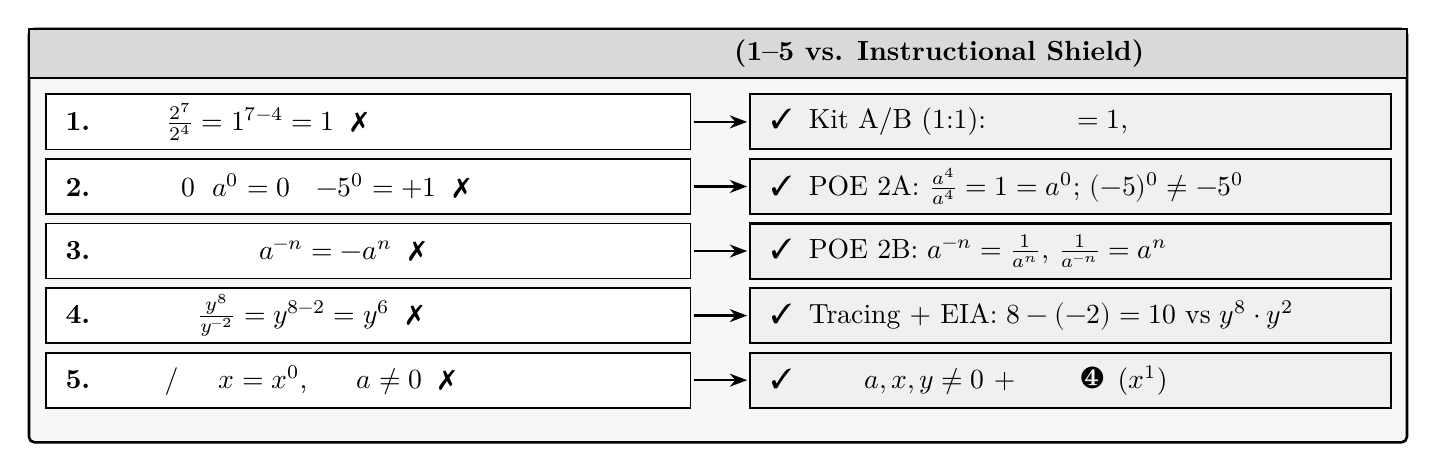
\begin{tikzpicture}[x=1cm, y=1cm, every node/.style={text=black, font=\fontsize{10pt}{13pt}\selectfont}]
  \draw[black, line width=0.95pt, fill=panelgray, rounded corners=2pt] (0,0) rectangle (17.50, 5.25);
  \node[anchor=center, fill=stepgray, draw=black, line width=0.7pt, minimum width=17.50cm, minimum height=0.62cm] at (8.75, 4.94)
    {\textbf{ផែនទីបង្ការកំហុសយល់ច្រឡំទាំង ៥ ផ្នែកនៃនិទស្សន្តរ៉ឺឡាទីប \en{(1--5 vs. Instructional Shield)}}};

  % ប្រអប់កំហុសខាងឆ្វេង ៥ ជួរ (x = 0.22 to 8.40)
  \draw[black, fill=white, line width=0.65pt] (0.22, 3.72) rectangle (8.40, 4.42);
  \node[anchor=west] at (0.34, 4.07) {\en{\textbf{1.}} ចែកគោល៖ $\frac{2^7}{2^4} = 1^{7-4} = 1$ \;\xkmark};

  \draw[black, fill=white, line width=0.65pt] (0.22, 2.90) rectangle (8.40, 3.60);
  \node[anchor=west] at (0.34, 3.25) {\en{\textbf{2.}} និទស្សន្ត $0$៖ $a^0 = 0$ ឬ $-5^0 = +1$ \;\xkmark};

  \draw[black, fill=white, line width=0.65pt] (0.22, 2.08) rectangle (8.40, 2.78);
  \node[anchor=west] at (0.34, 2.43) {\en{\textbf{3.}} និទស្សន្តអវិជ្ជមាន៖ $a^{-n} = -a^n$ \;\xkmark};

  \draw[black, fill=white, line width=0.65pt] (0.22, 1.26) rectangle (8.40, 1.96);
  \node[anchor=west] at (0.34, 1.61) {\en{\textbf{4.}} ដករ៉ឺឡាទីប៖ $\frac{y^8}{y^{-2}} = y^{8-2} = y^6$ \;\xkmark};

  \draw[black, fill=white, line width=0.65pt] (0.22, 0.44) rectangle (8.40, 1.14);
  \node[anchor=west] at (0.34, 0.79) {\en{\textbf{5.}} ភ្លេចដែន/គោល៖ $x = x^0$, ខ្វះ $a\neq 0$ \;\xkmark};

  % ព្រួញភ្ជាប់ទាំង ៥
  \foreach \yy in {4.07, 3.25, 2.43, 1.61, 0.79}{
    \draw[-{Stealth[length=2.2mm]}, line width=0.8pt, black] (8.44, \yy) -- (9.12, \yy);
  }

  % ខែលការពារខាងស្ដាំ ៥ ជួរ (x = 9.16 to 17.30)
  \draw[black, fill=headgray, line width=0.75pt] (9.16, 3.72) rectangle (17.30, 4.42);
  \node[anchor=west] at (9.30, 4.07) {\ckmark\; \en{Kit A/B (1:1)}: គូដូចគ្នា $=1$, គោលដដែល};

  \draw[black, fill=headgray, line width=0.75pt] (9.16, 2.90) rectangle (17.30, 3.60);
  \node[anchor=west] at (9.30, 3.25) {\ckmark\; \en{POE 2A}: $\frac{a^4}{a^4}=1=a^0$; $(-5)^0\neq -5^0$};

  \draw[black, fill=headgray, line width=0.75pt] (9.16, 2.08) rectangle (17.30, 2.78);
  \node[anchor=west] at (9.30, 2.43) {\ckmark\; \en{POE 2B}: $a^{-n}=\frac{1}{a^n}$, $\frac{1}{a^{-n}}=a^n$};

  \draw[black, fill=headgray, line width=0.75pt] (9.16, 1.26) rectangle (17.30, 1.96);
  \node[anchor=west] at (9.30, 1.61) {\ckmark\; \en{Tracing + EIA}: $8-(-2)=10$ vs $y^8\cdot y^2$};

  \draw[black, fill=headgray, line width=0.75pt] (9.16, 0.44) rectangle (17.30, 1.14);
  \node[anchor=west] at (9.30, 0.79) {\ckmark\; ប្រអប់ $a,x,y\neq 0$ + ហេតុផល \cnum{4} ($x^1$)};
\end{tikzpicture}
\end{center}
\figcap{១}{ការផ្គូផ្គងកំហុសយល់ច្រឡំទាំង ៥ ចំណុចពីអត្ថបទស្រាវជ្រាវ \en{[PDF 01--05]} ទៅនឹងយន្តការការពារក្នុងម៉ោង ៥០ នាទី}

% ============================================================================
% ផ្នែកទី ២៖ ទ្រឹស្ដីគរុកោសល្យ និងការបម្លែងភស្តុតាង ១៥ ឯកសារចូលក្នុងថ្នាក់ 5Es
% ============================================================================
\secbanner{២. ទ្រឹស្ដីគរុកោសល្យ និងការបម្លែងភស្តុតាង ១៥ ឯកសារចូលក្នុងថ្នាក់ \enbf{5Es}}{Section 2: Pedagogical Theory \& Translating All 15 Research Papers into 50-Min 5Es}

\subsec{២.១ ស្ថាបត្យកម្មគរុកោសល្យ៖ \enbf{5Es}, \enbf{POE}, គុណភាពការគិត និងស-ខ្មៅ \enbf{[tracing]}}
កញ្ចប់មេរៀន \en{POW23} សំយោគទ្រឹស្ដីគរុកោសល្យអន្តរជាតិ ៤ ស្រទាប់ឱ្យដំណើរការជាធ្លុងមួយក្នុងរយៈពេល ៥០ នាទីគត់៖
\begin{enumerate}[leftmargin=1.6em, itemsep=3pt, topsep=2pt]
  \item \textbf{លំហូរ \en{5Es} ស្ថាបនានិយម (\en{Polanin et al., 2024 [PDF 09]; Leton et al., 2026 [PDF 06]})៖} ការវិភាគមេតាលើការសិក្សា \en{RCT} ចំនួន ៦១ (\en{156 effect sizes}) របស់ \en{Polanin et al. (2024)} បង្ហាញឥទ្ធិពលវិជ្ជមាននៃគំរូ \en{5E} លើគណិតវិទ្យា ($k=6, m=9: g=0.70, 95\%\ \text{\en{CI}}\ [0.31, 1.10]$; ទោះលទ្ធផលវិភាគភាពរសើបថយមក $g=0.38$ ពី $1.09$ ក៏នៅតែវិជ្ជមាន)។ ចំពោះសិស្សថ្នាក់ទី៨ ផ្នែកស្វ័យគុណ \en{Leton et al. (2026)} ($N=72$) រកឃើញថាសកម្មភាពទាក់ទងបរិបទជាក់ស្ដែងជំរុញអក្ខរកម្មគណិតវិទ្យាពី $58.72$ ទៅ $82.57$ ($t(71)=20.63, p<.001, d_z=2.43, N\text{-gain}=0.60$)។ ដោយអនុវិទ្យាល័យព្រះក្រសាំងពុំប្រើអេក្រង់ \en{AR} ក្នុងថ្នាក់ធម្មតា យើងបម្លែងខ្លឹមសារជាបេសកកម្មកុំព្យូទ័រសាលា (\en{E1}) និងបន្ទះកាត់ \en{1:1} ជាក់ស្ដែងវិញ (\en{E2a})។
  \item \textbf{ពិសោធន៍ \en{POE} និងទំនាក់ទំនងសមាមាត្រ \en{Covariation} (\en{Jim\'enez-Valverde et al., 2026 [PDF 10]; Ellis et al., 2013 [PDF 07]})៖} \en{Jim\'enez-Valverde et al. (2026)} សំយោគការសិក្សា \en{POE (Predict--Observe--Explain)} ចំនួន ១២៨ ក្នុងវិទ្យាសាស្ត្រដែលយើងសម្របចូលគណិតវិទ្យាដោយឱ្យសិស្ស \textbf{ទស្សន៍ទាយមុន ($\frac{a^4}{a^4}, \frac{a^2}{a^4}$)} រួចផ្ទៀងផ្ទាត់ការលុបកត្តា។ ស្របគ្នា \en{Ellis et al. (2013)} ($N=3$ ថ្នាក់ទី៨, $92\%$ \en{IRR}) បង្ហាញថាការមើលលំនាំ $\div a$ តាមជណ្ដើរនិទស្សន្ត ($y_2/y_1=b^{x_2-x_1}$) ជួយឱ្យសិស្សទាញអត្ថន័យ $a^0=1$ និង $a^{-n}=\frac{1}{a^n}$ ដោយតក្កវិទ្យា មិនមែនចាំមាត់ទេ។
  \item \textbf{សញ្ញាសម្គាល់ស-ខ្មៅ \en{[tracing]} និងការបកស្រាយដោយខ្លួនឯង \cnum{1}--\cnum{5} (\en{Yeo \& Tzeng, 2019 [PDF 11]; Vest et al., 2022 [PDF 12]})៖} \en{Yeo \& Tzeng (2019)} ($N=72$, អាយុ ១១--១៣ ឆ្នាំ លើសំណួរបន្ទាត់ស្រប) បង្ហាញថាការភ្ជាប់រូបភាពតាមជំហាន \en{[tracing]} លើកកម្ពស់ការផ្ទេរចំណេះ ($M=3.00$ ទល់នឹង $2.31, p=.003, \eta^2=.121$) និងកាត់បន្ថយការលំបាក ($p\le .003$) ស្មើភាពគ្នាគ្រប់កម្រិតសមត្ថភាពចងចាំការងារ ($p\ge .447$)។ ដើម្បីឱ្យព្រីនស-ខ្មៅបាន ១០០\% យើងសម្របការហាយឡាយពណ៌ទៅជា \textbf{ប្រអប់ទ្វេ (មេគុណ), បន្ទាត់១ជាន់+រង្វង់ដាច់ (អថេរ $x$ និង $x^1$), និងបន្ទាត់២ជាន់ (អថេរ $y$)}។ លើសពីនេះ \en{Vest et al. (2022)} ($N=167$ ថ្នាក់ទី៦--៨, $36$ នាក់ថ្នាក់ទី៨) បញ្ជាក់ថាការបកស្រាយហេតុផលលើឧទាហរណ៍គំរូបង្កើនការយល់គំនិត ($\beta=1.23, p=.008$), ជំនាញវិធីសាស្ត្រ ($\beta=0.28, p=.022$) និងបន្ថយកំហុស ($\beta=-0.34, p=.004$)។ ដូច្នេះធនាគារហេតុផល \cnum{1}--\cnum{5} ត្រូវភ្ជាប់ជាប់នឹង \en{E4} និង \en{E5}។
  \item \textbf{ព្រំដែនសហការ និងកម្រិតឧទាហរណ៍ខុស (\en{Wang et al., 2026 [PDF 15]; Ngu et al., 2025 [PDF 14]})៖} \en{Wang et al. (2026)} ($N=134$ ថ្នាក់ទី៥ លើពហុកោណ) ព្រមានថាការធ្វើការជាក្រុមដោយគ្មានការចែកតួនាទីច្បាស់លាស់អាចបង្កើនបន្ទុកគិតដល់សិស្សមានមូលដ្ឋានទាប ($p<.05$ អន្តរកម្ម ៣ ទិស) តែបន្ថយបន្ទុកគិតពេលមានការណែនាំល្អ ($p<.01$) --- ទើប \en{Triad Relay} បែងចែក \textbf{តួនាទី ១--៣} ច្បាស់លាស់។ ចំណែក \en{Ngu et al. (2025)} (ថ្នាក់ទី៨ $N=68$ លើសមីការដឺក្រេទី១) បង្ហាញថាការដាក់ឧទាហរណ៍ត្រឹមត្រូវលាយខុស (\en{CICWE}) ក្នុងដំណាក់កាលហាត់អនុវត្តចម្បងបន្ថយការលើកទឹកចិត្ត ($p=.04$) និងបង្កផលប៉ះពាល់បញ្ច្រាសសម្រាប់សិស្សពូកែ ($p=.02$) --- ហេតុនេះយើង \textbf{មិន} ដាក់លំហាត់ខុសក្នុង \en{E4} ទេ តែប្រើវាត្រឹម \en{E5 Exit Foils A--D} រយៈពេល ៦០--៩០ វិនាទី ជាមួយការកែភ្លាមដើម្បីវាស់រោគវិនិច្ឆ័យ។
\end{enumerate}

\subsec{២.២ តារាងបម្លែងភស្តុតាងទាំង ១៥ ឯកសារ (\enbf{Evidence-to-Action Matrix})}

{\linespread{1.0}\fontsize{10.2pt}{15.5pt}\selectfont
\renewcommand{\arraystretch}{1.18}
\begin{longtable}{|L{2.30cm}|L{4.55cm}|L{5.10cm}|L{4.90cm}|}
\hline
\rowcolor{headgray}
\tblhead{លេខ \enbf{PDF /} អ្នកនិពន្ធ} & \tblhead{សំណាក និងលក្ខខណ្ឌសិក្សា} & \tblhead{លទ្ធផលជាក់ស្ដែងពីអត្ថបទ} & \tblhead{ការបម្លែងចូលក្នុង \enbf{50 min 5Es}} \\
\hline
\endfirsthead
\hline
\rowcolor{headgray}
\tblhead{លេខ \enbf{PDF /} អ្នកនិពន្ធ} & \tblhead{សំណាក និងលក្ខខណ្ឌសិក្សា} & \tblhead{លទ្ធផលជាក់ស្ដែងពីអត្ថបទ} & \tblhead{ការបម្លែងចូលក្នុង \enbf{50 min 5Es}} \\
\hline
\endhead
\en{[01] Ulusoy (2019)} & ថ្នាក់ទី៨ ($N=165$, សម្ភាសន៍ $12$ នាក់) លើនិទស្សន្តរ៉ឺឡាទីប។ & ត្រូវទាំងអស់ $4$ នាក់ ($3.5\%$); \en{Q1} $22.4\%$ ត្រូវ; \en{Q9} $17.0\%$ ត្រូវ; $>65\%$ ក្រោម ៣ ពិន្ទុ។ & កសាង \en{E2a (Kit A/B)} ទប់កំហុស $\frac{a^m}{a^n}=1^{m-n}$ និង \en{E2b} កែ $a^0=0$, $a^{-n}=-a^n$។ \\
\hline
\en{[02] Olson et al. (2011)} & និស្សិត ($N=904$, សម្ភាសន៍ $19$ នាក់) លើសញ្ញាដក។ & $5/19$ គិត $(-17)^8>-17^8$; $6/19$ ថា «វង់ក្រចកមិនសំខាន់ទេ»។ & បន្ថែមប្រអប់ $(-5)^0$ \en{vs} $-5^0$ ក្នុង \en{E2b} និង $(-2)^6$ \en{vs} $-2^6$ ក្នុង \en{E4}។ \\
\hline
\en{[03] Rohmah et al. (2023)} & ថ្នាក់ទី១០ ($N=29$, សម្ភាសន៍ $6$) វិភាគកំហុសស្វ័យគុណ។ & កំហុសគំនិត $52.29\%$, ភាសា $48.85\%$, បច្ចេកទេស $56.32\%$។ & បញ្ជាក់ពាក្យ«គោល, និទស្សន្ត, លក្ខខណ្ឌ $a\neq 0$» ក្នុង \en{E3} និងរំលឹក ២.២។ \\
\hline
\en{[04] \c{S}enay (2024)} & ពិនិត្យការសិក្សា ៥ ($N=729, 159, 69, 50, 50$)។ & សិស្សបន្ថយអរូបិយភាព \en{(reducing abstraction)} ជំនួសស្វ័យគុណដោយគុណធម្មតា។ & ប្រើបន្ទះ \en{1:1} ឱ្យឃើញកត្តាគុណពិតមុនរួមចេញរូបមន្តអរូបិយ $a^{m-n}$ ក្នុង \en{E3}។ \\
\hline
\en{[05] Suarka \& Kusumah (2024)} & សិស្ស $N=9$ (វិធីសាស្រ្តទំ. ៥៣២ ថាថ្នាក់ទី១១; ចំណងជើងថានិស្សិត)។ & $5/9$ ខុស $3^0$; $4/9$ ខុស $4^{-3}$; $6/9$ ខុស $-(2)^{-2}$; $7/9$ ខុស $-(2)^0$។ & បង្ខំឱ្យមានសំណួរ ៣០ វិនាទី (១--៦) ក្រោយ \en{POE 2A--2B} ដើម្បីបង្ក្រាបកំហុស $-(2)^0$។ \\
\hline
\en{[06] Leton et al. (2026)} & ថ្នាក់ទី៨ ($N=72$) អក្ខរកម្មគណិតវិទ្យាផ្នែកស្វ័យគុណ។ & ពិន្ទុកើន $58.72\to 82.57$, $t(71)=20.63, p<.001, d_z=2.43, N\text{-gain}=0.60$។ & សម្របបទពិសោធន៍ជាក់ស្ដែងជំនួស \en{AR} មកជាបញ្ហាកុំព្យូទ័រសាលា \en{E1} និងកាត់បន្ទះ \en{1:1}។ \\
\hline
\en{[07] Ellis et al. (2013)} & ថ្នាក់ទី៨ ($N=3$, $92\%$ \en{IRR}) សិក្សា \en{covariation}។ & សមាមាត្រគោល $y_2/y_1=b^{x_2-x_1}$ ជួយឱ្យសិស្សកសាងនិទស្សន្ត $0$ និងអវិជ្ជមាន។ & រចនាជណ្ដើរនិទស្សន្ត ($\div a$ ពី $a^3\to a^{-2}$) ក្នុង \en{POE 2B} សន្លឹកទី២។ \\
\hline
\en{[08] Slavit (2006)} & ថ្នាក់ទី៧--៨ ($N=30, 15$ គូ) ការសង្កេតលក្ខណៈពីជគណិត។ & $2/15$ គូសង្កេតភ្លាម បូក $6$ គូទៀតចាប់បានក្រោយគ្រូសួរដេញដោល។ & បង្កើត \en{Pause-Ask!} លើ ខ ($-\frac{9}{4}$ \en{vs} $\frac{4}{9}$) និង \en{Pause-Review!} លើ ឃ ($1$)។ \\
\hline
\en{[09] Polanin et al. (2024)} & វិភាគមេតា ៦១ \en{RCTs (156 ES)}; គណិត $k=6, m=9$។ & \en{5E} ផ្តល់ $g=0.70\ [0.31, 1.10]$ លើគណិតវិទ្យា (ភាពរសើប $1.09$ \en{vs} $0.38$)។ & រក្សាស្លាក \en{E1--E5} ឱ្យមានកាតព្វកិច្ចរកឃើញដោយសិស្សមុនបញ្ចូលទ្រឹស្ដី \en{E3}។ \\
\hline
\en{[10] Jim\'enez-Valverde et al. (2026)} & ពិនិត្យអត្ថបទ \en{POE} វិទ្យាសាស្ត្រ ១២៨ ពី ២១៥ អត្ថបទ។ & ជំហានទស្សន៍ទាយ--សង្កេត--បកស្រាយជួយបកអាក្រាតគំនិតខុសមុនពេលពន្យល់។ & សម្របមកគណិតវិទ្យាជាសន្លឹក \en{POE 2A--2B} (ទាយប្រអប់ចម្លើយមុនពិនិត្យលំហាត់)។ \\
\hline
\en{[11] Yeo \& Tzeng (2019)} & ក្មេងអាយុ ១១--១៣ ឆ្នាំ ($N=72$) \en{tracing} លំហាត់គំរូ។ & ផ្ទេរចំណេះខ្ពស់ $M=3.00$ \en{vs} $2.31, p=.003, \eta^2=.121$, ស្មើគ្រប់ \en{WMC} ($p\ge .447$)។ & បំប្លែងពណ៌មកសញ្ញាស-ខ្មៅ \en{[tracing]} ៣ ប្រភេទក្នុង \en{E4} គំរូ គ។ \\
\hline
\en{[12] Vest et al. (2022)} & ថ្នាក់ទី៦--៨ ($N=167, 36$ ថ្នាក់ទី៨) លើ \en{ITS} ពីជគណិត។ & ពន្យល់ខ្លួនឯងបង្កើនគំនិត ($\beta=1.23, p=.008$), វិធី ($\beta=0.28$), បន្ថយកំហុស ($\beta=-0.34$)។ & បង្កើតធនាគារហេតុផល \cnum{1}--\cnum{5} សម្រាប់សិស្សជ្រើសដាក់លើ \en{E4} និង \en{E5}។ \\
\hline
\en{[13] Pramasdyahsari et al. (2024)} & ថ្នាក់ទី១០ ($n=30, KR\text{-}20=0.6131$) តេស្ត ៣ ស្រទាប់។ & រកឃើញការយល់ច្រឡំ $55.17\%$ ($11\%$ វិជ្ជមានក្លែងក្លាយ, $44.1\%$ អវិជ្ជមានក្លែងក្លាយ)។ & ពិនិត្យភាពស៊ីគ្នារវាងចម្លើយ និងហេតុផល \cnum{1}--\cnum{5} ក្នុង \en{E5 Exit Foils}។ \\
\hline
\en{[14] Ngu et al. (2025)} & ថ្នាក់ទី៤ ($N=43$) និងថ្នាក់ទី៨ ($N=68$) សមីការដឺក្រេទី១។ & \en{CICWE} មិនឈ្នះ \en{WE/PS}, ទឹកចិត្តធ្លាក់ ($p=.04$), បញ្ច្រាសជំនាញ ($p=.02$)។ & \textbf{ហាម} ដាក់ឧទាហរណ៍ខុសក្នុង \en{E4}; ទុកជា \en{Exit Foils A--D} រហ័ស ៦០--៩០ វិនាទីតែប៉ុណ្ណោះ។ \\
\hline
\en{[15] Wang et al. (2026)} & ថ្នាក់ទី៥ ($N=134$) សហការជាមួយឧទាហរណ៍គំរូ។ & អន្តរកម្ម ៣ ទិស $p<.05$; ជួយក្រុមមូលដ្ឋានខ្ពស់ ($F=6.74, p<.05$) និងបន្ថយ \en{CL} ($p<.01$)។ & ចាត់តួនាទី \en{Triad Relay} ៣ មុខច្បាស់លាស់ កុំឱ្យសិស្សមានមូលដ្ឋានទាបអង្គុយស្ងៀម។ \\
\hline
\end{longtable}}

% ----------------------------------------------------------------------------
% រូបទី ២៖ ដ្យាក្រាមលំហូរ 5Es 50 នាទី (TikZ >= 10pt B&W)
% ----------------------------------------------------------------------------
\Needspace{6.3cm}
\begin{center}
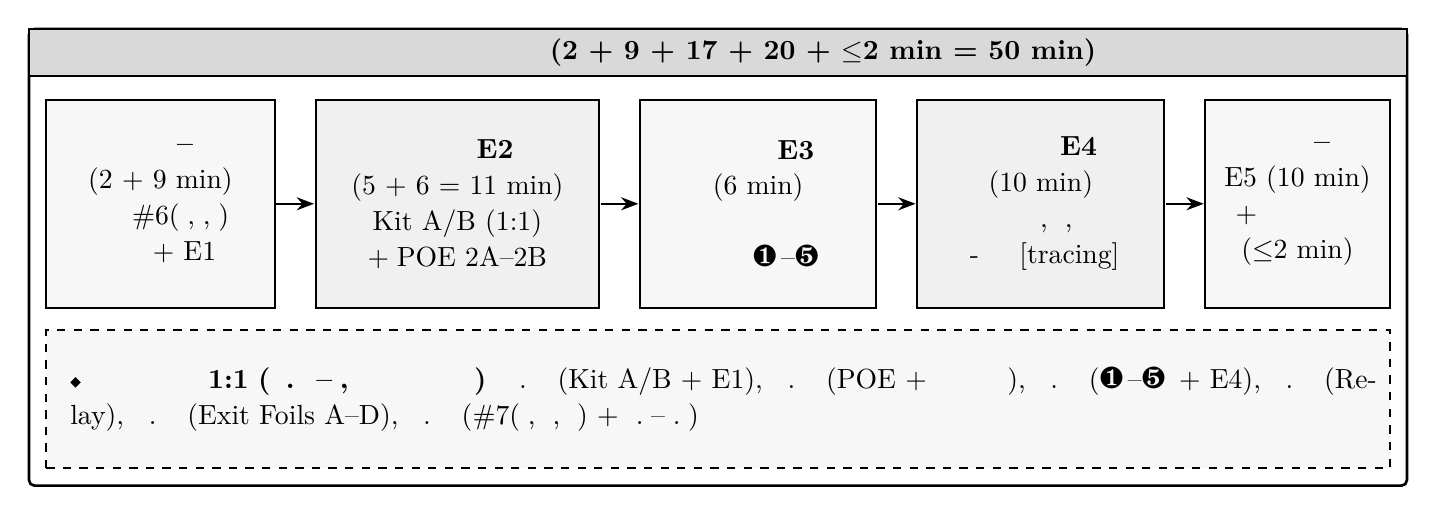
\begin{tikzpicture}[x=1cm, y=1cm, every node/.style={text=black, font=\fontsize{10pt}{13pt}\selectfont}]
  \draw[black, line width=0.95pt, fill=white, rounded corners=2pt] (0,0) rectangle (17.50, 5.80);
  \node[anchor=center, fill=stepgray, draw=black, line width=0.7pt, minimum width=17.50cm, minimum height=0.60cm] at (8.75, 5.50)
    {\textbf{ស្ថាបត្យកម្មលំហូរ ៥០ នាទី \en{(2 + 9 + 17 + 20 + $\le$2 min = 50 min)}}};

  % ប្រអប់ជំហាន ១-៥ (y = 2.26 to 4.90, កម្ពស់ 2.64 cm ធានាចន្លោះលើ-ក្រោមស្អាត)
  \draw[black, fill=panelgray, line width=0.75pt] (0.22, 2.26) rectangle (3.12, 4.90);
  \node[align=center, inner sep=3pt] at (1.67, 3.58) {\textbf{ជំហាន ១--២}\\(\en{2 + 9 min})\\កំណែ \en{\#6(}ក,ខ,គ\en{)}\\រំលឹក \en{+ E1}};

  \draw[-{Stealth[length=2.2mm]}, line width=0.85pt] (3.14, 3.58) -- (3.62, 3.58);

  \draw[black, fill=headgray, line width=0.75pt] (3.64, 2.26) rectangle (7.24, 4.90);
  \node[align=center, inner sep=3pt] at (5.44, 3.58) {\textbf{ជំហាន ៣៖ \en{E2}}\\(\en{5 + 6 = 11 min})\\\en{Kit A/B (1:1)}\\+\;\en{POE 2A--2B}};

  \draw[-{Stealth[length=2.2mm]}, line width=0.85pt] (7.26, 3.58) -- (7.74, 3.58);

  \draw[black, fill=panelgray, line width=0.75pt] (7.76, 2.26) rectangle (10.76, 4.90);
  \node[align=center, inner sep=3pt] at (9.26, 3.58) {\textbf{ជំហាន ៣៖ \en{E3}}\\(\en{6 min})\\បង្គុំច្បាប់ទាំង ៣\\ធនាគារ \cnum{1}--\cnum{5}};

  \draw[-{Stealth[length=2.2mm]}, line width=0.85pt] (10.78, 3.58) -- (11.26, 3.58);

  \draw[black, fill=headgray, line width=0.75pt] (11.28, 2.26) rectangle (14.42, 4.90);
  \node[align=center, inner sep=3pt] at (12.85, 3.58) {\textbf{ជំហាន ៤៖ \en{E4}}\\(\en{10 min})\\គំរូ ក, ខ, គ\\ស-ខ្មៅ \en{[tracing]}};

  \draw[-{Stealth[length=2.2mm]}, line width=0.85pt] (14.44, 3.58) -- (14.92, 3.58);

  \draw[black, fill=panelgray, line width=0.75pt] (14.94, 2.26) rectangle (17.28, 4.90);
  \node[align=center, inner sep=3pt] at (16.11, 3.58) {\textbf{ជំហាន ៤--៥}\\\en{E5 (10 min)}\\+ កិច្ចការផ្ទះ\\(\en{$\le$2 min})};

  % ប្រអប់ភ្ជាប់សន្លឹកបោះពុម្ពទំព័រ ១-៦ ខាងក្រោម
  \draw[black, dashed, line width=0.75pt, fill=panelgray] (0.22, 0.22) rectangle (17.28, 1.98);
  \node[anchor=west, text width=16.70cm, align=left] at (0.40, 1.10)
    {\ditem \textbf{សន្លឹកបោះពុម្ព \en{1:1} (ទំ. ១--៦, ចែកតាមដំណាក់កាល)៖} ទំ. ១ (\en{Kit A/B + E1}), ទំ. ២ (\en{POE} + ៣០ វិនាទី), ទំ. ៣ (\cnum{1}--\cnum{5} + \en{E4}), ទំ. ៤ (\en{Relay}), ទំ. ៥ (\en{Exit Foils A--D}), ទំ. ៦ (\en{\#7(}គ, ឃ, ច\en{)} + ៤.១--៤.២)។};
\end{tikzpicture}
\end{center}
\figcap{២}{ខ្សែសង្វាក់បង្រៀន ៥០ នាទី និងការផ្គូផ្គងទៅកាន់សន្លឹកកិច្ចការ \en{1:1} ទាំង ៦ ទំព័រ}

% ============================================================================
% ផ្នែកទី ៣៖ សៀវភៅណែនាំអនុវត្តលម្អិតតាមជំហាន ៥០ នាទី និងពាក្យគ្រូនិយាយផ្ទាល់
% ============================================================================
\secbanner{៣. សៀវភៅណែនាំអនុវត្តលម្អិតតាមជំហាន ៥០ នាទី និងពាក្យគ្រូនិយាយផ្ទាល់}{Section 3: Step-by-Step 50-Minute Execution Guide \& Verbatim Teacher Scripts}

គោលការណ៍ស្នូលក្នុងផ្នែកនេះគឺការបង្រៀនតាមបែប \textbf{ពាក្យគ្រូនិយាយផ្ទាល់} (\en{verbatim teacher voice}) ដែលសង្កត់ធ្ងន់លើការស្ដាប់គំនិតសិស្សមុនបូកសរុប និងការពារពេលវេលាឱ្យសល់គ្រប់គ្រាន់សម្រាប់ \en{E4} (១០ នាទី) និង \en{E5} (១០ នាទី)។

\begin{phasebox}{ជំហានទី ១៖ រដ្ឋបាលថ្នាក់ និងការរៀបចំក្រុម ៣ នាក់ \enbf{(Classroom Setup)}}{២ នាទី}
\begin{itemize}[leftmargin=1.4em, itemsep=2pt, topsep=1pt, label=\ditem]
  \item \textbf{សម្ភារៈត្រូវចែកតាមដំណាក់កាល (\en{Progressive Handout})៖} នៅជំហានទី ១ គ្រូចែកតែ \textbf{ទំព័រ ១} នៃ \en{Printable\_Materials\_POW23} (សន្លឹក \en{E1} និងបន្ទះកាត់ \en{1:1 Kit A--B} ដែលកាត់ទុកជាមុន) \textbf{ដាក់ផ្កាប់មុខលើតុ} សម្រាប់ក្រុម ៣ នាក់ (\en{Triad})។ ឯទំព័រ ២--៦ (\en{POE}, ធនាគារ \cnum{1}--\cnum{5}/\en{E4}, \en{Triad Relay}, \en{Exit Foils}, កិច្ចការផ្ទះ) ត្រូវកាន់ទុកហើយចែកបន្តបន្ទាប់តាមដំណាក់កាលនីមួយៗ។
  \item \textbf{ការគ្រប់គ្រងវិន័យ៖} ពិនិត្យអវត្តមានរហ័សក្នុង ៦០ វិនាទី និងហាមក្រុមត្រឡប់សន្លឹកទំព័រ ១ មុនសញ្ញា \en{E1}។
\end{itemize}
\end{phasebox}

\begin{scriptbox}[(ជំហានទី ១ \en{--} បើកម៉ោងសិក្សា)]
«សួស្ដីប្អូនៗទាំងអស់គ្នា! ថ្ងៃនេះយើងអង្គុយជាក្រុម ៣ នាក់មួយតុដើម្បីធ្វើបេសកកម្មជាក្រុមវិស្វករសាលាយើង។ សូមតំណាងក្រុមម្នាក់ទទួលសន្លឹក និងបន្ទះកាត់ \en{1:1} ទំព័រ ១ \textbf{ដាក់ផ្កាប់មុខលើតុសិន} កុំទាន់ត្រឡប់មើលឬកាត់អ្វីមុនសញ្ញារបស់គ្រូណា។ ប្រធានថ្នាក់ សូមជួយផ្ដល់ព័ត៌មានអវត្តមានរហ័សផង!»
\end{scriptbox}

\begin{phasebox}{ជំហានទី ២៖ កំណែកិច្ចការផ្ទះ រំលឹកមេរៀនចាស់ និង \enbf{E1 Engage}}{៩ នាទី \enbf{($\le$3 + 3 + 3)}}
\begin{itemize}[leftmargin=1.4em, itemsep=2pt, topsep=1pt, label=\ditem]
  \item \textbf{២.១ កំណែ ២.១ \en{\#6(}ក, ខ, គ\en{)} (\en{$\le$3 min})៖} កែតែ ៣ ចំណុចនេះប៉ុណ្ណោះ ($4^{11}$, $2^{15}$, $\frac{4}{3}$); \textbf{បិទមិនដាក់ \en{\#6.}ឃ} ព្រោះប្រើរូបមន្តមេរៀន ៤.២។ ដាក់បញ្ជាក់ពិសេសលើ ៦.ខ ដែលមានតួបង្កប់ $2 = 2^1$។
  \item \textbf{២.២ រំលឹកមូលដ្ឋាន (\en{3 min})៖} ប្រមូលចម្លើយមាត់រហ័សលើ (១) $a^n$ (និយមន័យស្វ័យគុណ), (២) $\frac{k}{k}=1$ ($k\neq 0$), (៣) $x=x^1$, និង (៤) វិធីដកចំនួនរ៉ឺឡាទីប $8-(-2)=8+2=10$ និង $2-4=-2$។
  \item \textbf{២.៣ \en{E1 -- Engage (3 min)}៖} ប្រធានបទ «ពង្រីកឃ្លាំងផ្ទុកឯកសារឌីជីថល \en{NGS}»៖ ឯកសារ ១ កញ្ចប់ $= 2^4\unit{MB}$។ បន្ទប់ \en{A} ($2^7\unit{MB}$), បន្ទប់ \en{B} ($2^4\unit{MB}$), បន្ទប់ \en{C} ($2^2\unit{MB}$)។ សិស្សត្រឡប់ទំ. ១ ឡើងទស្សន៍ទាយមុន (\en{Predict}) លើទំពក់ទាំង ៣៖ (១) $1^3$ ឬ $2^3$? (២) $0$ ឬ $1$? (៣) $-4$ ឬ $\frac{1}{4}$?
\end{itemize}
\end{phasebox}

\begin{scriptbox}[(ជំហានទី ២ \en{--} កំណែ និង \enbf{E1})]
«មើលទៅកំណែកិច្ចការ \en{\#6(}ក, ខ, គ\en{)} លើក្ដារខៀន៖ ក្នុង ៦.ខ តើលេខ $2$ នៅខាងមុខមាននិទស្សន្តអ្វីបង្កប់? បាទ! គឺ $2^1$ ដូច្នេះ $1+3+4+7=15$ បាន $2^{15}$។ ឯ \en{\#6.}ឃ យើងទុកសម្រាប់មេរៀនក្រោយ។ ឥឡូវត្រៀមខួរក្បាល៖ $\frac{k}{k}$ ($k\neq 0$) ស្មើប៉ុន្មាន? $x$ មាននិទស្សន្តអ្វីបង្កប់? $8-(-2)$ ស្មើប៉ុន្មាន? ចុះ $2-4$ ស្មើប៉ុន្មាន? ល្អណាស់! ស្ដាប់បេសកកម្មពិត៖ ឃ្លាំងផ្ទុកឯកសារឌីជីថលសាលាត្រូវរៀបកញ្ចប់ទំហំ $2^4\unit{MB}$។ បន្ទប់ \en{A} មាន $2^7\unit{MB}$, បន្ទប់ \en{B} មាន $2^4\unit{MB}$, បន្ទប់ \en{C} មាន $2^2\unit{MB}$។ សូមត្រឡប់សន្លឹកទំ. ១ ឡើង រួចគូសទាយសំណួរទំពក់ទាំង ៣ ក្នុង ៤៥ វិនាទី៖ (១) $2^7\div 2^4$ ស្មើ $1^3$ ឬ $2^3$? (២) $2^4\div 2^4$ ស្មើ $0$ ឬ $1$? (៣) $2^2\div 2^4$ ស្មើ $-4$ ឬ $\frac{1}{4}$? កុំទាន់ប្រាប់គ្នាថាត្រូវឬខុសណា!»
\end{scriptbox}

\begin{phasebox}{ជំហានទី ៣៖ \enbf{E2} (ពិសោធន៍ \enbf{1:1 + POE}) និង \enbf{E3} (ច្បាប់ \cnum{1}--\cnum{5})}{១៧ នាទី \enbf{(11 [5+6] + 6)}}
\begin{itemize}[leftmargin=1.4em, itemsep=2pt, topsep=1pt, label=\ditem]
  \item \textbf{សកម្មភាព \en{E2a --} បន្ទះកាត់ \en{1:1 (5 min}, ទំ. ១)៖} ក្រុមផ្គូផ្គង \en{Kit A} ($\frac{2^7}{2^4}$, \textbf{៧ កត្តា} $= 7.00\unit{cm}$ ទល់នឹង \textbf{៤ កត្តា} $= 4.00\unit{cm}$, ព្រមទាំងកែសៀវភៅក្រសួងទំ. ១៦ ដែលបាត់ ១ កត្តា) និង \en{Kit B} ($\frac{3^7}{3^5}$, $7.00\unit{cm}$ ទល់នឹង $5.00\unit{cm}$), លុបគូ $\frac{2}{2}=1$ ចេញ នៅសល់ $2^3=8$ និង $3^2=9$។
  \item \textbf{សកម្មភាព \en{E2b -- POE 2A, 2B}, ជណ្ដើរនិទស្សន្ត និងតេស្ត ៣០ វិនាទី (\en{6 min}, ចែកទំ. ២)៖} ក្រោយចប់ \en{E2a} គ្រូចែកទំព័រ ២ ដើម្បីធ្វើ \en{POE 2A} ($\frac{a^4}{a^4}=1=a^0$, ប្រៀបធៀប $(-5)^0=1$ \en{vs} $-5^0=-1$), \en{POE 2B} ($\frac{a^2}{a^4}=\frac{1}{a^2}=a^{-2}$, $2^{-2}=\frac{1}{4}$, $\frac{1}{y^{-2}}=y^2$), អានជណ្ដើរ $\div a$ ($a^3\to a^{-2}$), និងប្រាប់មាត់រួមគ្នា ៦ សំណួរក្នុង ៣០ វិនាទី។
  \item \textbf{ដំណាក់កាល \en{E3 -- Explain (6 min}, ចែកទំ. ៣)៖} សិស្សតំណាងក្រុមបូកសរុបច្បាប់ទាំង ៣ ($a\neq 0,\ m,n\in\mathbb{Z}$), គ្រូពន្យល់ការកែសម្រួលលក្ខខណ្ឌ $m,n\neq 0$ របស់សៀវភៅក្រសួង និងចែកទំព័រ ៣ ដើម្បីចាក់សោធនាគារហេតុផល \cnum{1}--\cnum{5} មុនចូល \en{E4}។
\end{itemize}
\end{phasebox}

\begin{scriptbox}[(ជំហានទី ៣ \en{-- E2} ពិសោធន៍ និង \enbf{E3} បង្គុំច្បាប់)]
«លើកបន្ទះ \en{Kit A} ឡើង! រាប់កត្តា $2$ នៅភាគយកជាមួយគ្រូ៖ ១, ២, ៣, ៤, ៥, ៦, \textbf{៧ កត្តា}! ចំណាំទុកក្នុងសៀវភៅទំព័រ ១៦ បោះពុម្ពខ្វះ ១ កត្តា សូមប្អូនថែម $\times 2$ មួយទៀតឱ្យគ្រប់ ៧។ ពេលយើងដាក់គូ $\frac{2}{2}=1$ ទល់គ្នា ៤ គូ តើនៅសល់ $2$ ប៉ុន្មានកត្តា? បាទ ៣ កត្តា គឺ $2^3$ មិនមែន $1^3$ ទេណា ព្រោះ $1\times 1\times 1\times 1\times 2\times 2\times 2$ រក្សាគោល $2$ ដដែល! ឥឡូវចូល \en{POE 2A}: ប្រើប៊ិចទាយមុនថា $\frac{a^4}{a^4}$ ស្មើប៉ុន្មាន? បើប្រើដកនិទស្សន្តបាន $a^{4-4}=a^0$ តែលុបកត្តាដូចគ្នាបាន $1$ ដូច្នេះ $a^0=1$ ($a\neq 0$)។ ប្រយ័ត្ន! $(-5)^0$ វង់ក្រចកកាន់សញ្ញាដក ស្មើ $+1$ ឯ $-5^0$ ស្មើ $-(5^0)=-1$! តោះឆ្លើយមាត់ ៣០ វិនាទី ៦ សំណួរព្រមគ្នា! ល្អ \en{--} ឥឡូវជួយបង្គុំច្បាប់ទូទៅទាំង ៣ ជាមួយគ្រូលើក្ដារខៀន ដោយដាក់ $a\neq 0$ ជាប់ជានិច្ច និងប្រើលេខហេតុផល \cnum{1}--\cnum{5} លើទំព័រ ៣ ដើម្បីការពារចម្លើយរបស់យើង!»
\end{scriptbox}

% ----------------------------------------------------------------------------
% រូបទី ៣៖ ការបង្ហាញ E2a (7 កត្តា Kit A) + POE ជណ្ដើរនិទស្សន្ត + (-5)^0 vs -5^0
% ----------------------------------------------------------------------------
\Needspace{5.2cm}
\begin{center}
\begin{minipage}{\linewidth}
\centering
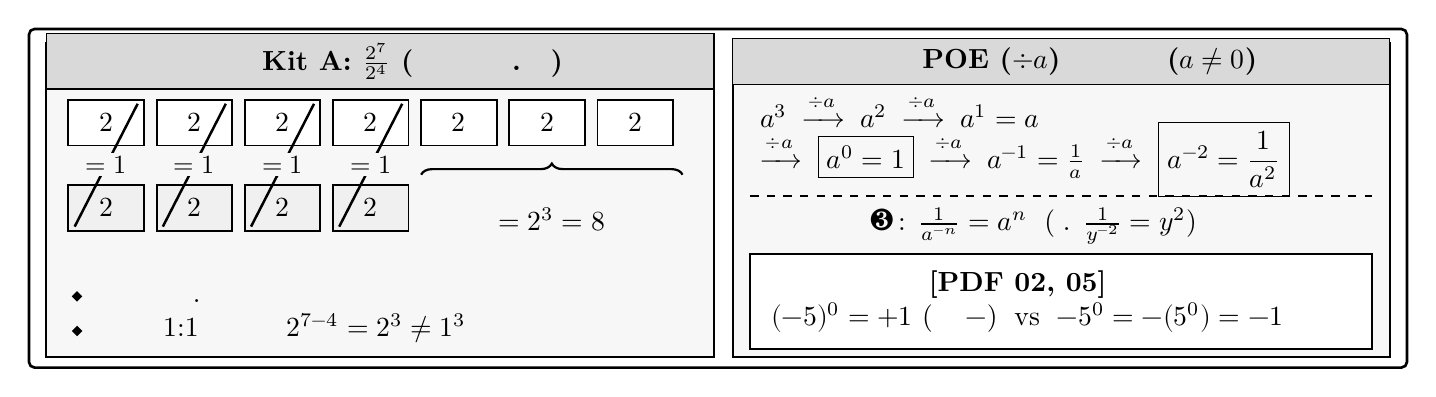
\begin{tikzpicture}[x=1cm, y=1cm, every node/.style={text=black, font=\fontsize{10pt}{12.5pt}\selectfont}]
  \draw[black, line width=0.95pt, fill=white, rounded corners=2pt] (0,0) rectangle (17.50, 4.30);

  % ប្រអប់ឆ្វេង៖ Kit A 7 កត្តា ទល់នឹង កំហុសទំព័រ ១៦
  \draw[black, fill=panelgray, line width=0.75pt] (0.22, 0.14) rectangle (8.70, 4.12);
  \node[anchor=center, fill=stepgray, draw=black, minimum width=8.48cm, minimum height=0.46cm] at (4.46, 3.89)
    {\textbf{ពិសោធន៍ \en{Kit A}: $\frac{2^7}{2^4}$ (\textbf{៧ កត្តា} កែទំ. ១៦)}};

  % ៧ ប្រអប់ភាគយក (y = 2.82 to 3.40)
  \foreach \i in {1,...,7}{
    \pgfmathsetmacro{\xx}{0.50 + (\i-1)*1.12}
    \draw[black, fill=white, line width=0.7pt] (\xx, 2.82) rectangle (\xx+0.96, 3.40);
    \node at (\xx+0.48, 3.11) {$2$};
  }
  % ៤ ប្រអប់ភាគបែង (y = 1.74 to 2.32)
  \foreach \i in {1,...,4}{
    \pgfmathsetmacro{\xx}{0.50 + (\i-1)*1.12}
    \draw[black, fill=headgray, line width=0.7pt] (\xx, 1.74) rectangle (\xx+0.96, 2.32);
    \node at (\xx+0.48, 2.03) {$2$};
    \draw[black, line width=0.9pt] (\xx+0.08, 1.79) -- (\xx+0.88, 3.35);
    \node[fill=panelgray, inner sep=1pt, font=\fontsize{9.5pt}{11pt}\selectfont] at (\xx+0.48, 2.58) {$=1$};
  }
  \draw[decorate, decoration={brace, amplitude=4pt}, line width=0.8pt] (4.98, 2.45) -- (8.30, 2.45);
  \node[anchor=north, align=center] at (6.64, 2.31) {សល់ \textbf{៣ កត្តា}\\$= 2^3 = 8$};
  \node[anchor=west, align=left] at (0.42, 0.64)
    {\ditem សៀវភៅក្រសួងទំ. ១៦ បោះពុម្ពតែ ៦ កត្តា\\
     \ditem ផ្គូផ្គង \en{1:1} ឃើញច្បាស់ $2^{7-4}=2^3\neq 1^3$};

  % ប្រអប់ស្ដាំ៖ ជណ្ដើរនិទស្សន្ត និងវង់ក្រចក
  \draw[black, fill=panelgray, line width=0.75pt] (8.94, 0.14) rectangle (17.28, 4.12);
  \node[anchor=center, fill=stepgray, draw=black, minimum width=8.34cm, minimum height=0.46cm] at (13.11, 3.89)
    {\textbf{ជណ្ដើរ \en{POE ($\div a$)} និងវង់ក្រចក ($a\neq 0$)}};

  \node[anchor=west] at (9.16, 3.24) {$a^3 \;\xrightarrow{\div a}\; a^2 \;\xrightarrow{\div a}\; a^1=a$};
  \node[anchor=west] at (9.16, 2.64) {$\xrightarrow{\div a}\; \boxed{a^0 = 1} \;\xrightarrow{\div a}\; a^{-1}=\frac{1}{a} \;\xrightarrow{\div a}\; \boxed{a^{-2}=\frac{1}{a^2}}$};
  \draw[black, dashed, line width=0.75pt] (9.16, 2.18) -- (17.06, 2.18);
  \node[anchor=west] at (9.16, 1.80) {\textbf{ច្បាប់ចម្រាស់} \cnum{3}: $\frac{1}{a^{-n}} = a^n$ \;(ឧ. $\frac{1}{y^{-2}}=y^2$)};
  \draw[black, fill=white, line width=0.7pt] (9.16, 0.24) rectangle (17.06, 1.44);
  \node[anchor=west, align=left] at (9.30, 0.84)
    {\textbf{ការពារកំហុសវង់ក្រចក \en{[PDF 02, 05]}៖}\\
     $(-5)^0 = +1$ (រួម $-$) \;\en{vs}\; $-5^0 = -(5^0) = -1$};
\end{tikzpicture}
\figcap{៣}{ការលុបកត្តា ៧ ទល់នឹង ៤ ក្នុង \en{Kit A (E2a)}, ជណ្ដើរ \en{POE} និង $(-5)^0$ \en{vs} $-5^0$ \en{(E2b)}}
\end{minipage}
\end{center}

\begin{phasebox}{ជំហានទី ៤៖ \enbf{E4 Elaborate} (ស-ខ្មៅ \enbf{[tracing] + EIA}) និង \enbf{E5 Evaluate}}{២០ នាទី \enbf{(10 + 10 [6+4])}}
\begin{itemize}[leftmargin=1.4em, itemsep=2pt, topsep=1pt, label=\ditem]
  \item \textbf{\en{E4 -- Elaborate (10 min}, ទំ. ៣)៖} បង្ហាញលំហាត់គំរូ ក ($\frac{10^8}{10^6}=10^2=100$) និង ខ ($\frac{(-2)^6}{(-2)^5}=(-2)^1=-2$ ភ្ជាប់ប្រអប់ $(-2)^6=64 \neq -2^6=-64$) ជាដំណើរការគិត។ បន្ទាប់មកអនុវត្ត \textbf{កាតស៊ើបអង្កេត ៣ ជំហានស-ខ្មៅ \en{[tracing]}} លើ គ ($\frac{\frac{5}{4}x^3 y^8}{-5xy^{-2}} = -\frac{1}{4}x^2 y^{10}$, $x,y\neq 0$) ដោយឱ្យសិស្សបំពេញចន្លោះ និងគូសធនាគារហេតុផល \cnum{1}--\cnum{5} ព្រមទាំងផ្ទៀងផ្ទាត់ \en{EIA Looking-Back} តាម ២ ផ្លូវ។
  \item \textbf{\en{E5 -- Triad Relay (6 min}, ចែកទំ. ៤)៖} ដោះស្រាយ ប្រតិបត្តិ ក--ឃ ($x^5$, $\frac{4}{9}$, $1$, $1$) ដោយប្ដូរវេន ៣ តួនាទី៖ \textbf{តួនាទី ១} (គូស \en{[tracing]} និងដាស់តឿន \en{Pause-Ask!}), \textbf{តួនាទី ២} (ដោះស្រាយ និងសរសេរ \cnum{1}--\cnum{5}), \textbf{តួនាទី ៣} (ផ្ទៀង \en{Pause-Review!} និងបិទបញ្ចប់បេសកកម្ម \en{E1}៖ \en{A:} ៨ កញ្ចប់, \en{B:} ១ កញ្ចប់, \en{C:} $\frac{1}{4}$ ថាស)។
  \item \textbf{\en{E5 -- Exit Foils A--D (4 min}, ចែកទំ. ៥)៖} ចែកកាត \en{Exit Foils A--D} (១ នាក់ ១ កាត កុំឱ្យមើលគ្នា); សិស្សឆ្លើយ \textbf{ត្រូវ/ខុស + ហេតុផល \cnum{1}--\cnum{5}} ក្នុង ៦០--៩០ វិនាទី រួចគ្រូបង្ហាញចម្លើយភ្លាម។ \textbf{ច្បាប់ $>20\%$៖} បើសិស្សខុសលើស $20\%$ (ឧ. ៥--៦ នាក់ឡើងទៅក្នុងថ្នាក់ ២៥--៣០ នាក់) គ្រូត្រូវពន្យល់ជួសជុលភ្លាម ២ នាទីមុនចេញពីថ្នាក់។
\end{itemize}
\end{phasebox}

\begin{scriptbox}[(ជំហានទី ៤ \en{-- E4} និង \enbf{E5})]
«មើលគំរូ គ៖ $\frac{\frac{5}{4}x^3 y^8}{-5xy^{-2}}$ មានទាំងលេខ ម៉ូណូម $x$ និង $y$ លាយគ្នា! កុំប្រញាប់ធ្វើ ឱ្យយើងប្រើវិធីស៊ើបអង្កេត \en{[tracing]} ទាំង ៣ ជំហានជាមួយគ្នា៖ ជំហានទី១ គូសប្រអប់ទ្វេព័ទ្ធមេគុណ $\frac{5/4}{-5}$, គូសបន្ទាត់ ១ ជាន់ក្រោម $x^3$ និង $x$ (ព័ទ្ធរង្វង់ដាច់លេខ \en{1} លើ $x^1$), គូសបន្ទាត់ ២ ជាន់ក្រោម $y^8$ និង $y^{-2}$! ជំហានទី២ ចែកតាមក្រុមគោល៖ $\frac{y^8}{y^{-2}}=y^{8-(-2)}=y^{10}$ ដោយហេតុផល \cnum{1} និង \cnum{4}! ជំហានទី៣ \en{EIA Looking-Back}: ប្រសិនបើយើងប្រើចម្រាស់ \cnum{3} វិញ គឺ $\frac{1}{y^{-2}}=y^2$ នោះ $y^8\cdot y^2 = y^{10}$ ដូចគ្នា! ឥឡូវទទួលសន្លឹកទំ. ៤ ចូល \en{Triad Relay} ៦ នាទី! តួនាទី ១ ឈប់សួរមិត្តភក្ដិត្រង់ \en{Pause-Ask!} នៃ ខ ហេតុអ្វី $\left(\frac{3}{2}\right)^{-2}$ មិនស្មើ $-\frac{9}{4}$ តែស្មើ $\frac{4}{9}$? ឯតួនាទី ៣ ពិនិត្យ \en{Pause-Review!} ត្រង់ ឃ ហេតុអ្វី $y$ នៅមុខ $x$ តែលទ្ធផលនៅតែ $1$ ($x,y\neq 0$)? ចុងក្រោយទុកសន្លឹកក្រុម រួចទទួលកាតតូច \en{Exit Foil} ម្នាក់មួយសន្លឹក ធ្វើស្ងាត់ៗ ៦០--៩០ វិនាទី!»
\end{scriptbox}

% ----------------------------------------------------------------------------
% រូបទី ៤៖ ការគូសស-ខ្មៅ [tracing] ក្នុង E4 និង EIA Looking-Back 2 ផ្លូវ (TikZ >= 10pt)
% ----------------------------------------------------------------------------
\Needspace{5.6cm}
\begin{center}
\begin{minipage}{\linewidth}
\centering
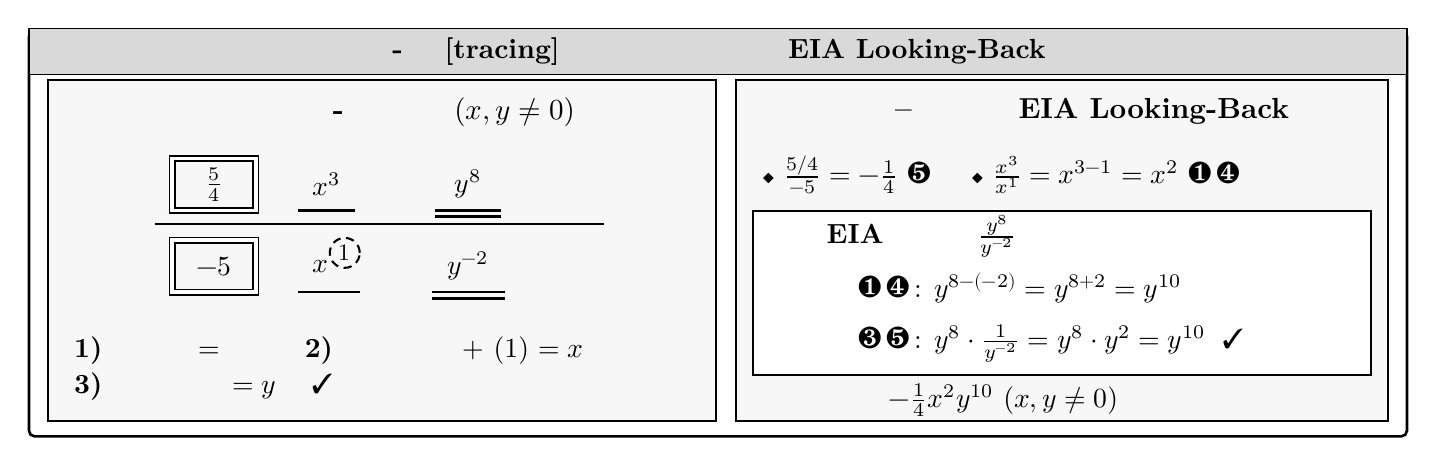
\begin{tikzpicture}[x=1cm, y=1cm, every node/.style={text=black, font=\fontsize{10pt}{13pt}\selectfont}]
  \draw[black, line width=0.95pt, fill=white, rounded corners=2pt] (0,0) rectangle (17.50, 5.15);
  \node[anchor=center, fill=stepgray, draw=black, minimum width=17.50cm, minimum height=0.52cm] at (8.75, 4.89)
    {\textbf{បច្ចេកទេសស-ខ្មៅ \en{[tracing]} ៣ ជំហាន និងការត្រួតពិនិត្យ \en{EIA Looking-Back} លើគំរូ គ}};

  % ផ្នែកឆ្វេង៖ រូបភាពកន្សោមគំរូ គ + ខ្សែបន្ទាត់ [tracing] (y = 0.20 to 4.52)
  \draw[black, fill=panelgray, line width=0.7pt] (0.24, 0.20) rectangle (8.72, 4.52);
  \node[anchor=north, font=\fontsize{10.5pt}{14pt}\selectfont] at (4.48, 4.42) {\textbf{ជំហានទី ១៖ ចំណាំស-ខ្មៅលើគំរូ គ} ($x,y\neq 0$)};

  % កន្សោមធំកណ្ដាល (y = 2.70)
  \draw[black, line width=0.8pt] (1.60, 2.70) -- (7.30, 2.70);
  % ភាគយក
  \draw[black, double distance=1.3pt, line width=0.6pt] (1.82, 2.87) rectangle (2.88, 3.53);
  \node at (2.35, 3.20) {$\frac{5}{4}$};
  \node at (3.78, 3.20) {$x^3$};
  \draw[black, line width=0.9pt] (3.42, 2.87) -- (4.14, 2.87);
  \node at (5.58, 3.20) {$y^8$};
  \draw[black, line width=0.9pt] (5.16, 2.87) -- (6.00, 2.87);
  \draw[black, line width=0.9pt] (5.16, 2.79) -- (6.00, 2.79);

  % ភាគបែង
  \draw[black, double distance=1.3pt, line width=0.6pt] (1.82, 1.83) rectangle (2.88, 2.49);
  \node at (2.35, 2.16) {$-5$};
  \node at (3.70, 2.16) {$x$};
  \draw[black, densely dashed, line width=0.75pt] (4.01, 2.33) circle (0.19);
  \node[font=\fontsize{8.5pt}{10pt}\selectfont] at (4.01, 2.33) {$1$};
  \draw[black, line width=0.9pt] (3.42, 1.83) -- (4.20, 1.83);
  \node at (5.58, 2.16) {$y^{-2}$};
  \draw[black, line width=0.9pt] (5.12, 1.83) -- (6.04, 1.83);
  \draw[black, line width=0.9pt] (5.12, 1.75) -- (6.04, 1.75);

  % ពន្យល់សញ្ញា ៣ ប្រភេទ
  \node[anchor=west, align=left] at (0.45, 0.86)
    {\en{\textbf{1)}} ប្រអប់ទ្វេ $=$ មេគុណ \quad \en{\textbf{2)}} បន្ទាត់ ១ ជាន់ $+$ \en{(1)} $= x$\\
     \en{\textbf{3)}} បន្ទាត់ ២ ជាន់ $= y$ \quad \ckmark\; គោលដូចគ្នាគូសដូចគ្នា};

  % ផ្នែកស្ដាំ៖ ជំហាន ២ និង ៣ EIA Looking-Back (y = 0.20 to 4.52)
  \draw[black, fill=panelgray, line width=0.7pt] (8.98, 0.20) rectangle (17.26, 4.52);
  \node[anchor=north, font=\fontsize{10.5pt}{14pt}\selectfont] at (13.12, 4.42) {\textbf{ជំហាន ២--៣៖ គណនា និង \en{EIA Looking-Back}}};
  \node[anchor=west] at (9.20, 3.32)
    {\ditem $\frac{5/4}{-5} = -\frac{1}{4}$ \cnum{5} \quad \ditem $\frac{x^3}{x^1} = x^{3-1} = x^2$ \cnum{1}\cnum{4}};

  % ប្រអប់សផ្ទៀង EIA ធំល្មមមិនប៉ះស៊ុម (y = 0.78 to 2.86)
  \draw[black, fill=white, line width=0.75pt] (9.20, 0.78) rectangle (17.04, 2.86);
  \node[anchor=west] at (9.38, 2.54) {\textbf{ផ្ទៀង \en{EIA} ២ ផ្លូវលើ $\frac{y^8}{y^{-2}}$៖}};
  \node[anchor=west] at (9.38, 1.88) {ផ្លូវទី ១ \cnum{1}\cnum{4}: $y^{8-(-2)} = y^{8+2} = y^{10}$};
  \node[anchor=west] at (9.38, 1.18) {ផ្លូវទី ២ \cnum{3}\cnum{5}: $y^8 \cdot \frac{1}{y^{-2}} = y^8 \cdot y^2 = y^{10}$ \;\ckmark};
  \node[anchor=west] at (9.20, 0.46) {\textbf{ចម្លើយចុងក្រោយ៖} $-\frac{1}{4}x^2 y^{10}$ ($x,y\neq 0$)};
\end{tikzpicture}
\figcap{៤}{ការបម្លែង \en{[tracing]} ពណ៌ \en{[PDF 11]} ជាសញ្ញាសម្គាល់ស-ខ្មៅ និង \en{EIA Looking-Back} ក្នុង \en{E4}}
\end{minipage}
\end{center}

\begin{phasebox}{ជំហានទី ៥៖ កិច្ចការផ្ទះ និងការអានត្រៀមមេរៀនបន្ទាប់}{$\le$២ នាទី}
\begin{itemize}[leftmargin=1.4em, itemsep=2pt, topsep=1pt, label=\ditem]
  \item \textbf{កិច្ចការផ្ទះផ្លូវការ (ទំ. ២៥)៖} ចែកប័ណ្ណទំព័រ ៦៖ \textbf{លំហាត់ទី ៧ (គ, ឃ, ច)} ($a,b,x\neq 0$)។ \textbf{ហាមដាក់ \en{\#7.}ង} (ជាមេរៀន ៤.១--៤.២ ដូច \en{\#6.}ឃ) ហើយប្រើអក្សរខ្មែរ \textbf{«៧.ច»} ត្រឹមត្រូវតាមទំព័រ ២៥ នៃសៀវភៅក្រសួង (មានផ្ទៀងផ្ទាត់អក្សរលំដាប់ គ, ឃ, ង, ច)។
  \item \textbf{អានត្រៀមមេរៀនក្រោយ៖} ចំណុច \textbf{៤. លក្ខណៈនៃស្វ័យគុណ (៤.១--៤.២, ទំព័រ ១៧--១៨)}។
\end{itemize}
\end{phasebox}

\begin{scriptbox}[(ជំហានទី ៥ \en{--} បិទម៉ោង)]
«សូមទទួលប័ណ្ណកិច្ចការផ្ទះតូចម្នាក់មួយសន្លឹក! យកទៅធ្វើលំហាត់ទី \textbf{៧ (គ, ឃ, ច)} ទំព័រ ២៥ ដោយសរសេរលក្ខខណ្ឌ $a,b,x\neq 0$ ផង។ ប្រយ័ត្នណា៖ កុំធ្វើ ៧.ង ឱ្យសោះព្រោះយើងមិនទាន់រៀន ៤.១--៤.២ ទេ ហើយកត់ចំណាំសរសេរលេខ \textbf{៧.ច} ឱ្យបានត្រឹមត្រូវតាមសៀវភៅ (ក្នុងប័ណ្ណមានប្រធានពេញស្រាប់)។ សូមអានចំណុច ៤. លក្ខណៈនៃស្វ័យគុណ (៤.១--៤.២, ទំព័រ ១៧--១៨) ទុកជាមុនសម្រាប់ម៉ោងក្រោយ។ អរគុណប្អូនៗ!»
\end{scriptbox}

% ============================================================================
% ផ្នែកទី ៤៖ ការគ្រប់គ្រងសម្ភារៈបោះពុម្ព ១:១ ប្លង់ក្ដារខៀន និងដោះស្រាយបញ្ហាជាក់ស្ដែង
% ============================================================================
\secbanner{៤. ការគ្រប់គ្រងសម្ភារៈបោះពុម្ព \enbf{1:1} ប្លង់ក្ដារខៀន និងការដោះស្រាយបញ្ហា}{Section 4: 1:1 Printables Management, Board Blueprint \& Troubleshooting}

\subsec{៤.១ បទប្បញ្ញត្តិបោះពុម្ព \enbf{Actual Size 100\%} និងការចែកសន្លឹក ៦ ទំព័រ}
សន្លឹកកិច្ចការ \en{Printable\_Materials\_POW23.pdf} មាន ៦ ទំព័រគូរដោយទំហំស-ខ្មៅពិតប្រាកដ៖
\begin{itemize}[leftmargin=1.4em, itemsep=2pt, topsep=1pt, label=\ditem]
  \item \textbf{ការផ្ទៀងផ្ទាត់មាត្រដ្ឋាន \en{1:1} (ទំ. ១)៖} នៅពេលព្រីនត្រូវជ្រើស \en{\textbf{Actual Size / Scale 100\%}} (\textbf{ហាម} ប្រើ \en{Fit to Page})។ ប្រើបន្ទាត់វាស់បន្ទះ \en{Calibration Bar 5.00 cm} លើទំព័រ ១; ប្រសិនបើខុសពី $4.9\text{--}5.1\unit{cm}$ សូមកែការកំណត់ព្រីនធ័រ ឬឱ្យសិស្សរាប់ប្រអប់ $1\unit{cm}$ ផ្ទាល់ជំនួសការវាស់ប្រវែងសុទ្ធ។
  \item \textbf{កាលវិភាគចែកតាមដំណាក់កាល (\en{Progressive Handout})៖} ទំព័រ ១ (\en{E1} + បន្ទះកាត់ \en{Kit A/B}) ចែក \textbf{ផ្កាប់មុខលើតុ} នៅជំហានទី ១ (១ ឈុតក្នុង ១ ក្រុម ៣ នាក់); ទំព័រ ២ ចែកពេលចូល \en{E2b}; ទំព័រ ៣ ចែកពេលចូល \en{E3/E4}; ទំព័រ ៤ ចែកពេល \en{E5 Triad Relay}; ទំព័រ ៥ (កាត់ជា ៤ កាត \en{Exit Foils A--D}) ចែកពេលបញ្ចប់ \en{Relay} ដល់នាទីទី ៤៤; និងទំព័រ ៦ (កាត់ ៤ ប័ណ្ណ) ចែកនៅ ១--២ នាទីចុងក្រោយ។
\end{itemize}

\subsec{៤.២ ប្លង់ក្ដារខៀនស្តង់ដារ ៣ ប្រឡោះ \enbf{(Board Layout Blueprint)}}

{\linespread{1.0}\fontsize{10.2pt}{15.2pt}\selectfont
\renewcommand{\arraystretch}{1.15}
\begin{longtable}{|L{5.65cm}|L{5.75cm}|L{5.75cm}|}
\hline
\rowcolor{headgray}
\tblhead{ប្រឡោះទី ១ \enbf{(}ឆ្វេង\enbf{)}} &
\tblhead{ប្រឡោះទី ២ \enbf{(}កណ្ដាល\enbf{)}} &
\tblhead{ប្រឡោះទី ៣ \enbf{(}ស្ដាំ\enbf{)}} \\
\hline
\endfirsthead
\hline
\rowcolor{headgray}
\tblhead{ប្រឡោះទី ១ \enbf{(}ឆ្វេង\enbf{)}} &
\tblhead{ប្រឡោះទី ២ \enbf{(}កណ្ដាល\enbf{)}} &
\tblhead{ប្រឡោះទី ៣ \enbf{(}ស្ដាំ\enbf{)}} \\
\hline
\endhead
  \ditem កំណែ \en{\#6(}ក, ខ, គ\en{)} ($4^{11}, 2^{15}, \frac{4}{3}$); បិទ \en{\#6.}ឃ &
  \ditem ចំណងជើង៖ \textbf{២.៣ វិធីចែកស្វ័យគុណមាននិទស្សន្តរ៉ឺឡាទីប} &
  \ditem គំរូ \en{E4}: ក ($100$), ខ ($-2$) + $(-2)^6\neq -2^6$ \\
\hline
  \ditem រំលឹក៖ $a^n$, $\frac{k}{k}=1$, $x=x^1$, $8-(-2)=10$, $2-4=-2$ &
  \ditem \en{Kit A} ($\frac{2^7}{2^4}=2^3$, \textbf{៧ កត្តា}) \& \en{Kit B} ($3^2$) &
  \ditem គំរូ គ \en{[tracing]}: $-\frac{1}{4}x^2y^{10}$ + \en{EIA} ២ ផ្លូវ \\
\hline
  \ditem បេសកកម្ម \en{E1 (A, B, C)} &
  \ditem ជណ្ដើរ \en{POE}: $a^3\to a^{-2}$ + ច្បាប់ $a\neq 0$ &
  \ditem \en{Triad Relay}: ក ($x^5$), ខ ($\frac{4}{9}$), គ ($1$), ឃ ($1$) \\
\hline
  \ditem ធនាគារហេតុផល \cnum{1}--\cnum{5} &
  \ditem បិទបញ្ចប់ \en{E1}: $8$, $1$, $\frac{1}{4}$ ថាស &
  \ditem កិច្ចការផ្ទះ៖ \textbf{\en{\#7(}គ, ឃ, ច\en{)}} (ទំ. ២៥) + ៤.១--៤.២ \\
\hline
\end{longtable}}

\subsec{៤.៣ តារាងដោះស្រាយបញ្ហាជាក់ស្ដែងក្នុងថ្នាក់ \enbf{(If--Then Troubleshooting)}}

{\linespread{1.0}\fontsize{10.2pt}{15.5pt}\selectfont
\renewcommand{\arraystretch}{1.18}
\begin{longtable}{|L{4.95cm}|L{5.35cm}|L{6.85cm}|}
\hline
\rowcolor{headgray}
\tblhead{បញ្ហាដែលអាចកើតមានក្នុងថ្នាក់} & \tblhead{មូលហេតុគរុកោសល្យ / ប្រតិបត្តិ} & \tblhead{ដំណោះស្រាយភ្លាមរបស់គ្រូ \enbf{(Action Protocol)}} \\
\hline
\endfirsthead
\hline
\rowcolor{headgray}
\tblhead{បញ្ហាដែលអាចកើតមានក្នុងថ្នាក់} & \tblhead{មូលហេតុគរុកោសល្យ / ប្រតិបត្តិ} & \tblhead{ដំណោះស្រាយភ្លាមរបស់គ្រូ \enbf{(Action Protocol)}} \\
\hline
\endhead
\textbf{១. អស់ម៉ោងមុនដល់ \en{Exit Foils}} & ចំណាយលើស \en{3 min} លើកំណែ \en{\#6} ឬសិស្សកាត់ក្រដាស \en{Kit A/B} យឺត។ & កាត់បន្ទះទុកមុនជាស្រេច; ចំពោះកំណែ \en{\#6} ឱ្យសិស្សផ្ទៀងជាមួយក្ដារខៀនតែ ៣ នាទីគត់ ហាមសរសេរឡើងវិញយូរ។ \\
\hline
\textbf{២. សិស្សដកនិទស្សន្តភ្លាម មិនលុបកត្តា} & ទម្លាប់សូត្ររូបមន្តមុនពិសោធន៍ (\en{reducing abstraction})។ & សួរត្រឡប់៖ «ហេតុអ្វី $\frac{2^7}{2^4}$ មិនស្មើ $1^{7-4}$?» រួចបង្ខំឱ្យដាក់គូ $\frac{2}{2}=1$ លើ \en{Kit A} ឱ្យឃើញនឹងភ្នែក។ \\
\hline
\textbf{៣. សិស្សគិតថា $a^0 = 0$} & យល់ច្រឡំថា «ស្វ័យគុណសូន្យគ្មានកត្តា ស្មើសូន្យ»។ & បង្ហាញ $\frac{5^3}{5^3}$ ស្មើ $1$ (ចំនួនដូចគ្នាចែកគ្នា) មុនសរសេរ $5^{3-3}=5^0$ ដូច្នេះ $5^0=1$។ \\
\hline
\textbf{៤. សិស្សច្រឡំ $-5^0 = 1$ និង $(-5)^0$} & មិនស្គាល់វិសាលភាពវង់ក្រចក \en{[PDF 02, 05]}។ & បាំងសញ្ញាដកមុខ $-5^0$ ដោយម្រាមដៃសួរ $5^0=?$ រួចដកម្រាមដៃចេញជា $-(1)=-1$។ \\
\hline
\textbf{៥. ធ្វើខុសសញ្ញា $\frac{y^8}{y^{-2}} = y^6$} & ភ្លេចសញ្ញាដកពីរដងក្នុង $m-(-n)$។ & បង្ខំឱ្យសរសេរ $8 - \boxed{(-2)}$ មុនបំប្លែងជា $8+2$, រួចផ្ទៀងដោយ \cnum{3} គឺ $y^8\cdot y^2$។ \\
\hline
\textbf{៦. សិស្សខ្សោយស្ងៀមក្នុង \en{Triad Relay}} & ទុកឱ្យសិស្សពូកែធ្វើតែម្នាក់ឯង \en{[PDF 15]}។ & ផ្លាស់វេនតួនាទី ១$\to$២$\to$៣ តាមជួរ៖ សិស្សខ្សោយទទួល \textbf{តួនាទី ១} (គូស \en{[tracing]} និងសួរ \en{Pause-Ask!})។ \\
\hline
\textbf{៧. កាត \en{Exit Foils} ខុស $>20\%$} & ក្រុមហាក់ដូចចេះតាមគ្នា តែមិនទាន់យល់បុគ្គល \en{[PDF 13]}។ & ទុកកិច្ចការ ១ នាទីលើ ប្រតិបត្តិ មេរៀនក្រោយដោយជួសជុល ២ នាទីលើកាតដែលខុសច្រើន (ភាគច្រើន \en{B} ឬ \en{D})។ \\
\hline
\end{longtable}}

% ============================================================================
% ផ្នែកទី ៥៖ ឯកសារផ្ទៀងផ្ទាត់ចម្លើយផ្លូវការ និងដំណោះស្រាយលម្អិត
% ============================================================================
\secbanner{៥. ឯកសារផ្ទៀងផ្ទាត់ចម្លើយផ្លូវការ និងដំណោះស្រាយលម្អិត}{Section 5: Official Answer Key, Diagnostic Rubrics \& Homework Solutions}

\subsec{៥.១ ចម្លើយកិច្ចការចាស់ ២.១ \enbf{\#6(}ក, ខ, គ\enbf{)} និងសំណួរ ៣០ វិនាទី \enbf{E2b (}១--៦\enbf{)}}
\begin{itemize}[leftmargin=1.4em, itemsep=2pt, topsep=1pt, label=\ditem]
  \item \textbf{កិច្ចការចាស់ ២.១ \en{\#6} (ទំ. ២៥)៖}
  \textbf{៦.ក:} $(4^5)(4^2)(4^4) = 4^{5+2+4} = 4^{11}$ \;\en{|}\;
  \textbf{៦.ខ:} $2\times 2^3\times 2^4\times 2^7 = 2^{\boxed{1}+3+4+7} = 2^{15}$ \;\en{|}\;
  \textbf{៦.គ:} $\left(\frac{4}{3}\right)^4\left(\frac{4}{3}\right)^{-6}\left(\frac{4}{3}\right)^3 = \left(\frac{4}{3}\right)^1 = \frac{4}{3}$ (កុំដាក់ ៦.ឃ)។
  \item \textbf{តេស្តមាត់ ៣០ វិនាទី \en{E2b} (សន្លឹកទំ. ២)៖}
  \textbf{១)} $2^0 = 1$;\;
  \textbf{២)} $2^{-2} = \frac{1}{4}$;\;
  \textbf{៣)} $\frac{1}{5^{-2}} = 25$;\;
  \textbf{៤)} $(-7)^0 = 1$;\;
  \textbf{៥)} $-7^0 = -1$;\;
  \textbf{៦)} $\frac{y^8}{y^{-2}} = y^{10}$ ($y\neq 0$)។
\end{itemize}

\subsec{៥.២ ចម្លើយលម្អិត \enbf{E4}, \enbf{E5 Triad Relay} និងវិនិច្ឆ័យ \enbf{Exit Foils A--D}}

{\linespread{1.0}\fontsize{10.2pt}{15.5pt}\selectfont
\renewcommand{\arraystretch}{1.18}
\begin{longtable}{|L{2.95cm}|L{6.05cm}|L{3.10cm}|L{4.75cm}|}
\hline
\rowcolor{headgray}
\tblhead{លំហាត់ / កាត} & \tblhead{ដំណោះស្រាយ និងចម្លើយត្រឹមត្រូវ} & \tblhead{ហេតុផល \cnum{1}--\cnum{5}} & \tblhead{ចំណុចត្រួតពិនិត្យ / កែតម្រូវ} \\
\hline
\endfirsthead
\hline
\rowcolor{headgray}
\tblhead{លំហាត់ / កាត} & \tblhead{ដំណោះស្រាយ និងចម្លើយត្រឹមត្រូវ} & \tblhead{ហេតុផល \cnum{1}--\cnum{5}} & \tblhead{ចំណុចត្រួតពិនិត្យ / កែតម្រូវ} \\
\hline
\endhead
\textbf{\en{E4} គំរូ ក, ខ} & ក: $\frac{10^8}{10^6}=10^2=100$; ខ: $\frac{(-2)^6}{(-2)^5}=(-2)^1=-2$ & \cnum{1} & ប្រអប់ប្រៀបធៀប $(-2)^6=64 \neq -2^6=-64$។ \\
\hline
\textbf{\en{E4} គំរូ គ} & $\frac{\frac{5}{4}x^3 y^8}{-5xy^{-2}} = -\frac{1}{4}x^2 y^{10}$ ($x,y\neq 0$) & \cnum{5}, \cnum{1}, \cnum{4}, \cnum{3} & បំពេញ \en{[tracing]} ៣ ជំហាន + \en{EIA} $y^8\cdot y^2=y^{10}$។ \\
\hline
\textbf{\en{Relay} ប្រតិបត្តិ ក} & $\frac{x^9}{x^4} = x^{9-4} = x^5$ ($x\neq 0$) & \cnum{1} & ហាមភ្លេចលក្ខខណ្ឌ $x\neq 0$។ \\
\hline
\textbf{\en{Relay} ប្រតិបត្តិ ខ} & $\frac{\left(\frac{3}{2}\right)^2}{\left(\frac{3}{2}\right)^4} = \left(\frac{3}{2}\right)^{-2} = \frac{1}{(3/2)^2} = \frac{4}{9}$ & \cnum{1}, \cnum{3} & \textbf{\en{Pause-Ask!}} ហេតុអ្វីមិនស្មើ $-\frac{9}{4}$? (សញ្ញាដកនៅនិទស្សន្ត មិនមែនមុខលេខ)។ \\
\hline
\textbf{\en{Relay} ប្រតិបត្តិ គ} & $\frac{y^9}{y^9} = y^{9-9} = y^0 = 1$ ($y\neq 0$) & \cnum{1}, \cnum{2} & បញ្ជាក់លក្ខខណ្ឌ $y\neq 0$ និងចំនួនចែកខ្លួនឯងស្មើ $1$។ \\
\hline
\textbf{\en{Relay} ប្រតិបត្តិ ឃ} & $\left(\frac{3yx^9}{-15y^5x^4}\right)^0 = 1$ ($x,y\neq 0$) & \cnum{2} & \textbf{\en{Pause-Review!}} លំដាប់ $y$ មុន $x$; បើពន្លាតជា $\left(-\frac{x^5}{5y^4}\right)^0=1$។ \\
\hline
\textbf{\en{Exit Foil A}} & អះអាង $\frac{6^8}{6^2}=1^4=1$ $\to$ \textbf{ខុស} (\xkmark) & \cnum{1} & កែ៖ $\frac{6^8}{6^2}=6^{8-2}=6^6$ (គោលរក្សា $6$ ដដែល)។ \\
\hline
\textbf{\en{Exit Foil B}} & អះអាង $\frac{a^5}{a^{-3}}=a^2$ ($a\neq 0$) $\to$ \textbf{ខុស} (\xkmark) & \cnum{1}, \cnum{4} (ឬ \cnum{3}) & កែ៖ $a^{5-(-3)}=a^{5+3}=a^8$ (សញ្ញាដកពីរដង)។ \\
\hline
\textbf{\en{Exit Foil C}} & អះអាង $\frac{-8a^3b^{-2}}{2a^3b^{-5}}=-4b^3$ ($a,b\neq 0$) $\to$ \textbf{ត្រូវ} (\ckmark) & \cnum{5}, \cnum{1}, \cnum{2}, \cnum{4} & $-4 a^{3-3} b^{-2-(-5)} = -4 a^0 b^3 = -4b^3$។ \\
\hline
\textbf{\en{Exit Foil D}} & អះអាង $\left(\frac{-7a^4}{b^2}\right)^0=0$ ($a,b\neq 0$) $\to$ \textbf{ខុស} (\xkmark) & \cnum{2} & កែ៖ កន្សោមខុសពីសូន្យស្វ័យគុណ $0$ ស្មើ $1$ (មិនមែន $0$)។ \\
\hline
\end{longtable}}

\subsec{៥.៣ ដំណោះស្រាយលម្អិតកិច្ចការផ្ទះ \enbf{\#7(}គ, ឃ, ច\enbf{)} (ទំព័រ ២៥)}
សិស្សត្រូវបញ្ជាក់ដែនកំណត់ $a,b\neq 0$ ឬ $a,x\neq 0$ រាល់លំហាត់ទាំង ៣ ខាងក្រោម៖
\begin{enumerate}[leftmargin=1.6em, itemsep=3pt, topsep=2pt]
  \item \textbf{លំហាត់ ៧.គ (កាត ក)៖} $\displaystyle \frac{\left(\frac{3}{2}a^2b^3\right)(2a^{-3}b^4)}{6a^{-2}b^4} = \frac{3\,a^{-1}b^7}{6\,a^{-2}b^4} = \frac{1}{2}a^{-1-(-2)}b^{7-4} = \frac{1}{2}ab^3$ \quad ($a,b\neq 0$)។
  \item \textbf{លំហាត់ ៧.ឃ (កាត ខ)៖} $\displaystyle \frac{(32a^2x^8)(-5a^4x^3)}{5ax(-2a^2x^2)(-4a^3x)} = \frac{-160\,a^6 x^{11}}{40\,a^6 x^4} = -4\,a^{6-6}x^{11-4} = -4x^7$ \quad ($a,x\neq 0$)។
  \item \textbf{លំហាត់ ៧.ច (កាត គ, ទំព័រ ២៥)៖}
  $\displaystyle \frac{\left(\frac{3}{2}a^2b^3\right)^0(2a^{-3}b^5)}{6a^{-2}b^4} = \frac{1\cdot 2a^{-3}b^5}{6a^{-2}b^4} = \frac{1}{3}a^{-3-(-2)}b^{5-4} = \frac{1}{3}a^{-1}b = \frac{b}{3a}$ \quad ($a,b\neq 0$)។
\end{enumerate}

% ============================================================================
% ផ្នែកទី ៦៖ បញ្ជីផ្ទៀងផ្ទាត់ក្រោយបង្រៀន និងភាពស៊ីចង្វាក់នៃកញ្ចប់ឯកសារ ៥ ផ្នែក
% ============================================================================
\secbanner{៦. បញ្ជីផ្ទៀងផ្ទាត់ក្រោយបង្រៀន និងសន្ទស្សន៍ឯកសារ ៥ ផ្នែក}{Section 6: Post-Lesson Reflection Checklist \& 5-Part Package Verification}

\subsec{៦.១ កំណត់ត្រាឆ្លុះបញ្ចាំងរបស់គ្រូក្រោយបញ្ចប់ ៥០ នាទី}
\begin{calloutbox}{តារាងផ្ទៀងផ្ទាត់ខ្លួនឯងរបស់គ្រូ \enbf{(Teacher Post-Class Audit)}}
\begin{itemize}[leftmargin=1.4em, itemsep=2.5pt, topsep=1pt, label=\ditem]
  \item \textbf{ការគ្រប់គ្រងពេល ៥០ នាទី៖} តើបានរក្សាពេល \en{E4} ($10\unit{min}$) និង \en{E5} ($10\unit{min}$) ពេញលេញ ដោយមិនបណ្ដោយឱ្យកំណែ \en{\#6} ឬការកាត់ \en{Kit A/B} លើសម៉ោងទេ?
  \item \textbf{អត្រាជោគជ័យ \en{Exit Foils A--D}៖} តើកាតណា (\en{A, B, C, D}) មានអត្រាខុស $>20\%$? បើមាន កត់ចំណាំដើម្បីផ្ដើមម៉ោងក្រោយ ២ នាទីលើលក្ខណៈបង្គំ ៤.១--៤.២។
  \item \textbf{ភាពត្រឹមត្រូវនៃអថេរ និងលក្ខខណ្ឌ៖} តើសិស្សភាគច្រើនសរសេរ $a\neq 0$ និង $x,y\neq 0$ ដោយស្វ័យប្រវត្តិមុនចេញចម្លើយចុងក្រោយដែរឬទេ?
  \item \textbf{កិច្ចការ \en{\#7(}គ, ឃ, ច\en{)}៖} តើបានពិនិត្យថាគ្មានសិស្សធ្វើច្រឡំ \en{\#7.}ង និងយល់ហេតុផល \cnum{3} លើ ៧.ច ($\frac{1}{3}a^{-1}b=\frac{b}{3a}$) ដែរឬទេ?
\end{itemize}
\end{calloutbox}

\subsec{៦.២ សន្ទស្សន៍ផ្ទៀងផ្ទាត់ ១-ទល់-១ រវាងបញ្ជីយោង និងថត ឯកសារស្រាវជ្រាវយោង\enbf{\_PDF}}
ឯកសារយោង \en{APA 7th} ចំនួន ១៥ ខាងក្រោមត្រូវបានផ្ទៀងផ្ទាត់ ១-ទល់-១ ជាមួយឯកសារ \en{PDF} ពិតប្រាកដក្នុងថត ឯកសារស្រាវជ្រាវយោង\en{\_PDF\textbackslash} តាមលេខរៀងដូចតទៅ៖
\en{Ellis et al. (2013) [07]},
\en{Jim\'enez-Valverde et al. (2026) [10]},
\en{Leton et al. (2026) [06]},
\en{Ngu et al. (2025) [14]},
\en{Olson et al. (2011) [02]},
\en{Polanin et al. (2024) [09]},
\en{Pramasdyahsari et al. (2024) [13]},
\en{Rohmah et al. (2023) [03]},
\en{\c{S}enay (2024) [04]},
\en{Slavit (2006) [08]},
\en{Suarka \& Kusumah (2024) [05]},
\en{Ulusoy (2019) [01]},
\en{Vest et al. (2022) [12]},
\en{Wang et al. (2026) [15]},
និង \en{Yeo \& Tzeng (2019) [11]}។

% ============================================================================
% បញ្ជីឯកសារយោង APA 7th (ប្រើ \refbanner{ឯកសារយោង} ១ ជួរស្អាត ១០០%)
% ============================================================================
\refbanner{ឯកសារយោង}

{\TimesEn\linespread{1.0}\fontsize{10.8pt}{16.2pt}\selectfont
\begingroup
\setlength{\parindent}{0pt}
\setlength{\parskip}{3.5pt}

\hangindent=0.85cm\hangafter=1
Ellis, A. B., Ozgur, Z., Kulow, T., Dogan, M. F., Williams, C., \& Amidon, J. (2013). Correspondence and covariation: Quantities changing together. In M. Martinez \& A. Castro Superfine (Eds.), \textit{Proceedings of the 35th Annual Meeting of the North American Chapter of the International Group for the Psychology of Mathematics Education} (pp. 119--126). University of Illinois at Chicago. (ERIC Document No. ED584480). \url{https://files.eric.ed.gov/fulltext/ED584480.pdf}

\hangindent=0.85cm\hangafter=1
Jim\'enez-Valverde, G., Fabre-Mitjans, N., \& Mart\'in-Hern\'andez, E. (2026). Predict--Observe--Explain (POE) in science education: A narrative review of mechanisms, variants, evidence, and disciplinary adaptations. \textit{Encyclopedia}, \textit{6}(11), Article 242. \url{https://doi.org/10.3390/encyclopedia6110242}

\hangindent=0.85cm\hangafter=1
Leton, S. I., Lakapu, M., Jagom, Y. O., Djong, K. D., Dosinaeng, W. B. N., \& Kusuma, D. A. (2026). Integrating augmented reality and local wisdom in teaching exponents: A strategy to improve students' mathematical literacy. \textit{Infinity Journal}, \textit{15}(3), 901--920. \url{https://doi.org/10.22460/infinity.v15i3.p901-920}

\hangindent=0.85cm\hangafter=1
Ngu, B. H., Chen, O., Phan, H. P., Usop, H., \& Anding, P. N. (2025). Can correct and incorrect worked examples supersede worked examples and problem-solving on learning linear equations? An examination from cognitive load and motivation perspectives. \textit{Education Sciences}, \textit{15}(4), Article 504. \url{https://doi.org/10.3390/educsci15040504}

\hangindent=0.85cm\hangafter=1
Olson, J. C., Cangelosi, R., Madrid, S., Cooper, S., \& Hartter, B. (2011). Ambiguity of the negative sign. In L. R. Wiest \& T. Lamberg (Eds.), \textit{Proceedings of the 33rd Annual Meeting of the North American Chapter of the International Group for the Psychology of Mathematics Education} (pp. 113--120). University of Nevada, Reno. (ERIC Document No. ED585963). \url{https://files.eric.ed.gov/fulltext/ED585963.pdf}

\hangindent=0.85cm\hangafter=1
Polanin, J. R., Austin, M., Taylor, J. A., Steingut, R. R., Rodgers, M. A., \& Williams, R. (2024). Effects of the 5E Instructional Model: A systematic review and meta-analysis. \textit{AERA Open}, \textit{10}(1), 1--16. \url{https://doi.org/10.1177/23328584241269866}

\hangindent=0.85cm\hangafter=1
Pramasdyahsari, A. S., Viviana, D., Sugiyanti, S., Pant, B. P., \& Ratnayake, I. (2024). Construction of three-tier diagnostic test for identifying student misconceptions in exponential properties. \textit{Jurnal Riset Pendidikan Matematika}, \textit{11}(1), 64--76. \url{https://doi.org/10.21831/jrpm.v11i1.73561}

\hangindent=0.85cm\hangafter=1
Rohmah, S., Jannah, I., \& Qowiyuddin, A. (2023). Analysis of Madrasah Aliyah students' errors on exponent materials in view of students' mathematical ability levels. \textit{Journal of Mathematical Pedagogy}, \textit{4}(2), 106--119. \url{https://doi.org/10.26740/jomp.v4n2.p106-119}

\hangindent=0.85cm\hangafter=1
\c{S}enay, \c{S}. C. (2024). Analysis of misconceptions and errors regarding exponential and radical expressions through the theory of reducing abstraction. \textit{Research on Education and Psychology (REP)}, \textit{8}(2), 281--295. \url{https://doi.org/10.54535/rep.1520588}

\hangindent=0.85cm\hangafter=1
Slavit, D. (2006). Uncovering algebra: Sense making and property noticing. \textit{The Mathematics Educator}, \textit{16}(2), 4--13. (ERIC Document No. EJ844242). \url{https://files.eric.ed.gov/fulltext/EJ844242.pdf}

\hangindent=0.85cm\hangafter=1
Suarka, N. K. S. D., \& Kusumah, Y. S. (2024). Students' learning obstacles in exponential: A case study in Indonesian higher education students. \textit{Jurnal Pendidikan MIPA}, \textit{25}(2), 530--541. \url{https://doi.org/10.23960/jpmipa/v25i2.pp530-541}

\hangindent=0.85cm\hangafter=1
Ulusoy, F. (2019). Serious obstacles hindering middle school students' understanding of integer exponents. \textit{International Journal of Research in Education and Science (IJRES)}, \textit{5}(1), 52--69. (ERIC Document No. EJ1198050). \url{https://files.eric.ed.gov/fulltext/EJ1198050.pdf}

\hangindent=0.85cm\hangafter=1
Vest, N. A., Silla, E. M., Bartel, A. N., Nagashima, T., Aleven, V., \& Alibali, M. W. (2022). Self-explanation of worked examples integrated in an intelligent tutoring system enhances problem solving and efficiency in algebra. In J. Culbertson, A. Perfors, H. Rabagliati, \& V. Ramenzoni (Eds.), \textit{Proceedings of the 44th Annual Conference of the Cognitive Science Society} (pp. 3466--3472). Cognitive Science Society. (ERIC Document No. ED623402). \url{https://files.eric.ed.gov/fulltext/ED623402.pdf}

\hangindent=0.85cm\hangafter=1
Wang, Y., Li, Q., \& Liu, X. (2026). Boundary conditions of collaborative learning using worked-examples: Joint moderating effects of task-specific prior knowledge and task complexity on transfer performance and cognitive load. \textit{Frontiers in Psychology}, \textit{17}, Article 1855051. \url{https://doi.org/10.3389/fpsyg.2026.1855051}

\hangindent=0.85cm\hangafter=1
Yeo, L.-M., \& Tzeng, Y.-T. (2019). Tracing effect in the worked examples-based learning: An exploration of individual differences in working memory capacity. \textit{Eurasia Journal of Mathematics, Science and Technology Education}, \textit{15}(10), Article em1760. \url{https://doi.org/10.29333/ejmste/105482}

\endgroup}

% ============================================================================
% ហត្ថលេខា (Signature Block — Khmer Lunar & Solar Dates Synced)
% ============================================================================
\Needspace{3.6cm}
\vspace{4pt}
\begin{flushright}
{\linespread{1.2}\fontsize{11pt}{16pt}\selectfont
ថ្ងៃចន្ទ ៧កើត ខែកត្តិក ឆ្នាំមមី អដ្ឋស័ក ពុទ្ធសករាជ ២៥៧០\\
កំពង់ស្វាយ, ថ្ងៃទី១៦ ខែវិច្ឆិកា ឆ្នាំ២០២៦\\}
\vspace{2pt}
\end{flushright}
\begin{center}
  \hspace*{10.5cm}{\linespread{1.0}\muol\fontsize{11.5pt}{18pt}\selectfont គ្រូបង្រៀន}
\end{center}
\vspace{32pt}
\hfill{\linespread{1.0}\muol\fontsize{11.5pt}{18pt}\selectfont ហុក ប៊ុនថែន}\hspace*{1.4cm}

\end{document}
